\section{Simulering}

I dette afsnit laves simuleringen for det samlede kredsløb i 2. iteration. 
Selve simuleringsdokumentet er delt op i blokke for at gøre det mere overskueligt. 


\noindent Kigges der på det yderste trin på figur~\ref{fig: simtop}, ses blot indgangsspændingen på 26V og udgangsloaden, der er sat op til $8.4\ohm$.
\begin{figure}[H]
	\center
	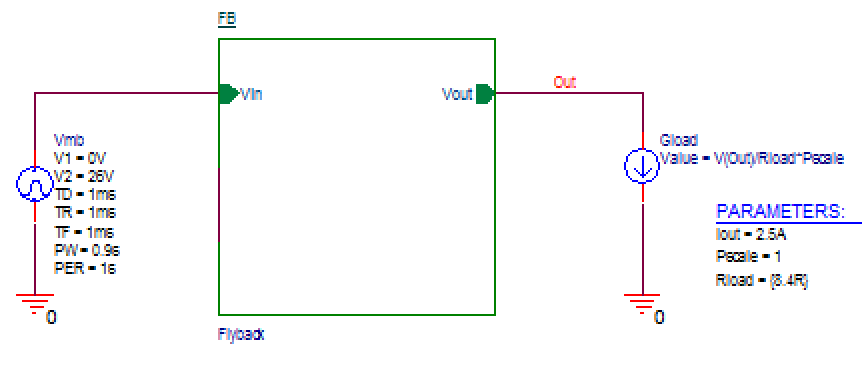
\includegraphics[max width=0.7\linewidth]{/tex/2iteration/billeder/Simulering_2iteration_top.png}
	\caption{Yderste blok af simulering}
	\label{fig: simtop}
\end{figure}
Imellem er blokken "Flyback". Heri er selve kredsløbet. Dykkes der ind i denne blok fås det der ses på figur~\ref{fig: simfly} 
\begin{figure}[H]
	\center
	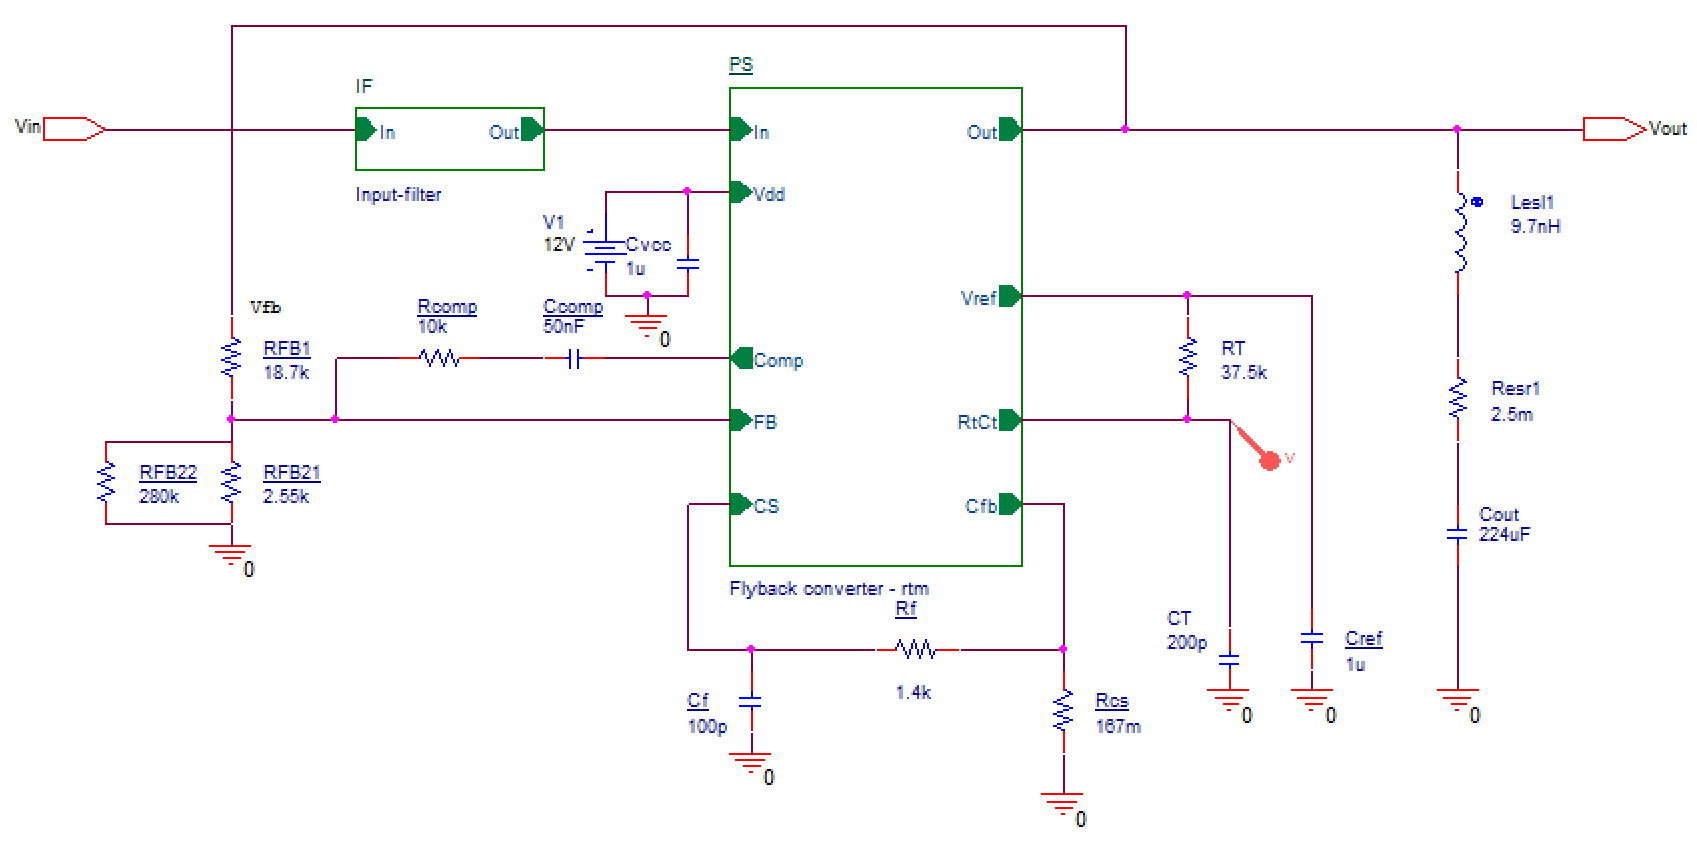
\includegraphics[max width=0.7\linewidth]{/tex/2iteration/billeder/Simulering_2iteration_flyback.png}
	\caption{Flyback blok}
	\label{fig: simfly}
\end{figure}
Her ses yderligere 2 blokke hhv. Inputfilter og flyback converter. Ud over disse blokke ses de komponenter, der er brugt til at få PWM controlleren til at køre efter hensigten. Selve controlleren ligger inde i flyback converter blokken. Værdierne og forklaringen af komponenterne blev gennemgået i analyse afsnittet om PWM controlleren??
Desuden ses output kondensatoren med de udregnede parasitter også.


\noindent Blokken for inputfiltret er allerede vist tidligere under forklaringen af denne, så den vises ikke igen. Til gengæld ses indholdet af Flyback converter blokken på figur~\ref{fig: simflycon}. 
\begin{figure}[H]
	\center
	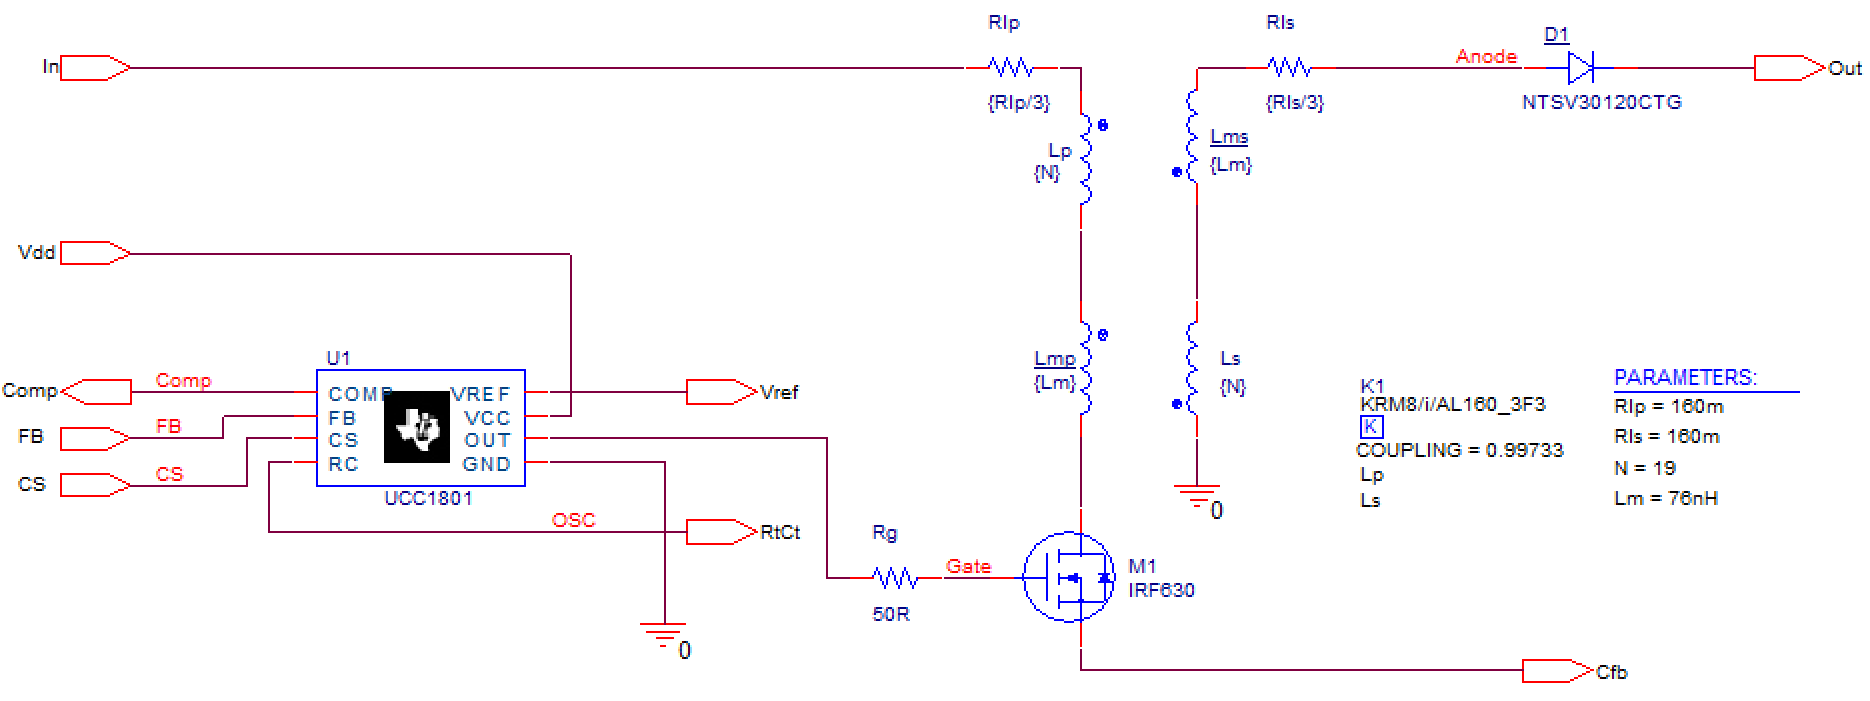
\includegraphics[max width=0.7\linewidth]{/tex/2iteration/billeder/Simulering_2iteration_flycon.png}
	\caption{Flyback converter blok}
	\label{fig: simflycon}
\end{figure}
Heri ses selve PWM controlleren UCC1801, som der er trukket en model ind for. \cite{??}. Også MOSFET'en og Dioden er der trukket modeller ind for. Ved MOSFET'en har det ikke været muligt at finde den præcise model. Derfor er IRF630 modellen istedet brugt, da det er vurderet, at den minder en del om den\cite{IRF630}. 
Yderligere ses transformatoren, hvor både spredningsselvinduktion og kobbermodstanden i ledningerne er tegnet med samt kernemodellen for 3F3 er trukket ind.

%%% Simulering af PWM-controller for 2. iteration

\subsection{PWM-controller}
I det følgende afsnit simuleres funktionaliteterne omkring PWM-controlleren. Her simuleres frekvensen af savtandspændingen og selve switch-frekvensen, samt signalet over current-sense modstanden både før og efter filteret.

\subsubsection{Switch-frekvens}
\noindent Først simuleres frekvensen af savtandspændingen. Dette er gjort på figur~\ref{fig:Simulering_PWM_savtand}. Periodetiden af savtandspændingen aflæses til $5.01\micro s$. Omregnet til en frekvens giver det: $f_{osc}=\frac{1}{5.01\micro s}=199.6k\hertz$. Derudover aflæses signalets minimumsspænding til ca. $138mV$, og maksimum- til ca. $2.5V$. I følge teorien burde spændingen ligge mellem $200mV$ og $2.65V$.

\begin{figure}[H]
	\center
	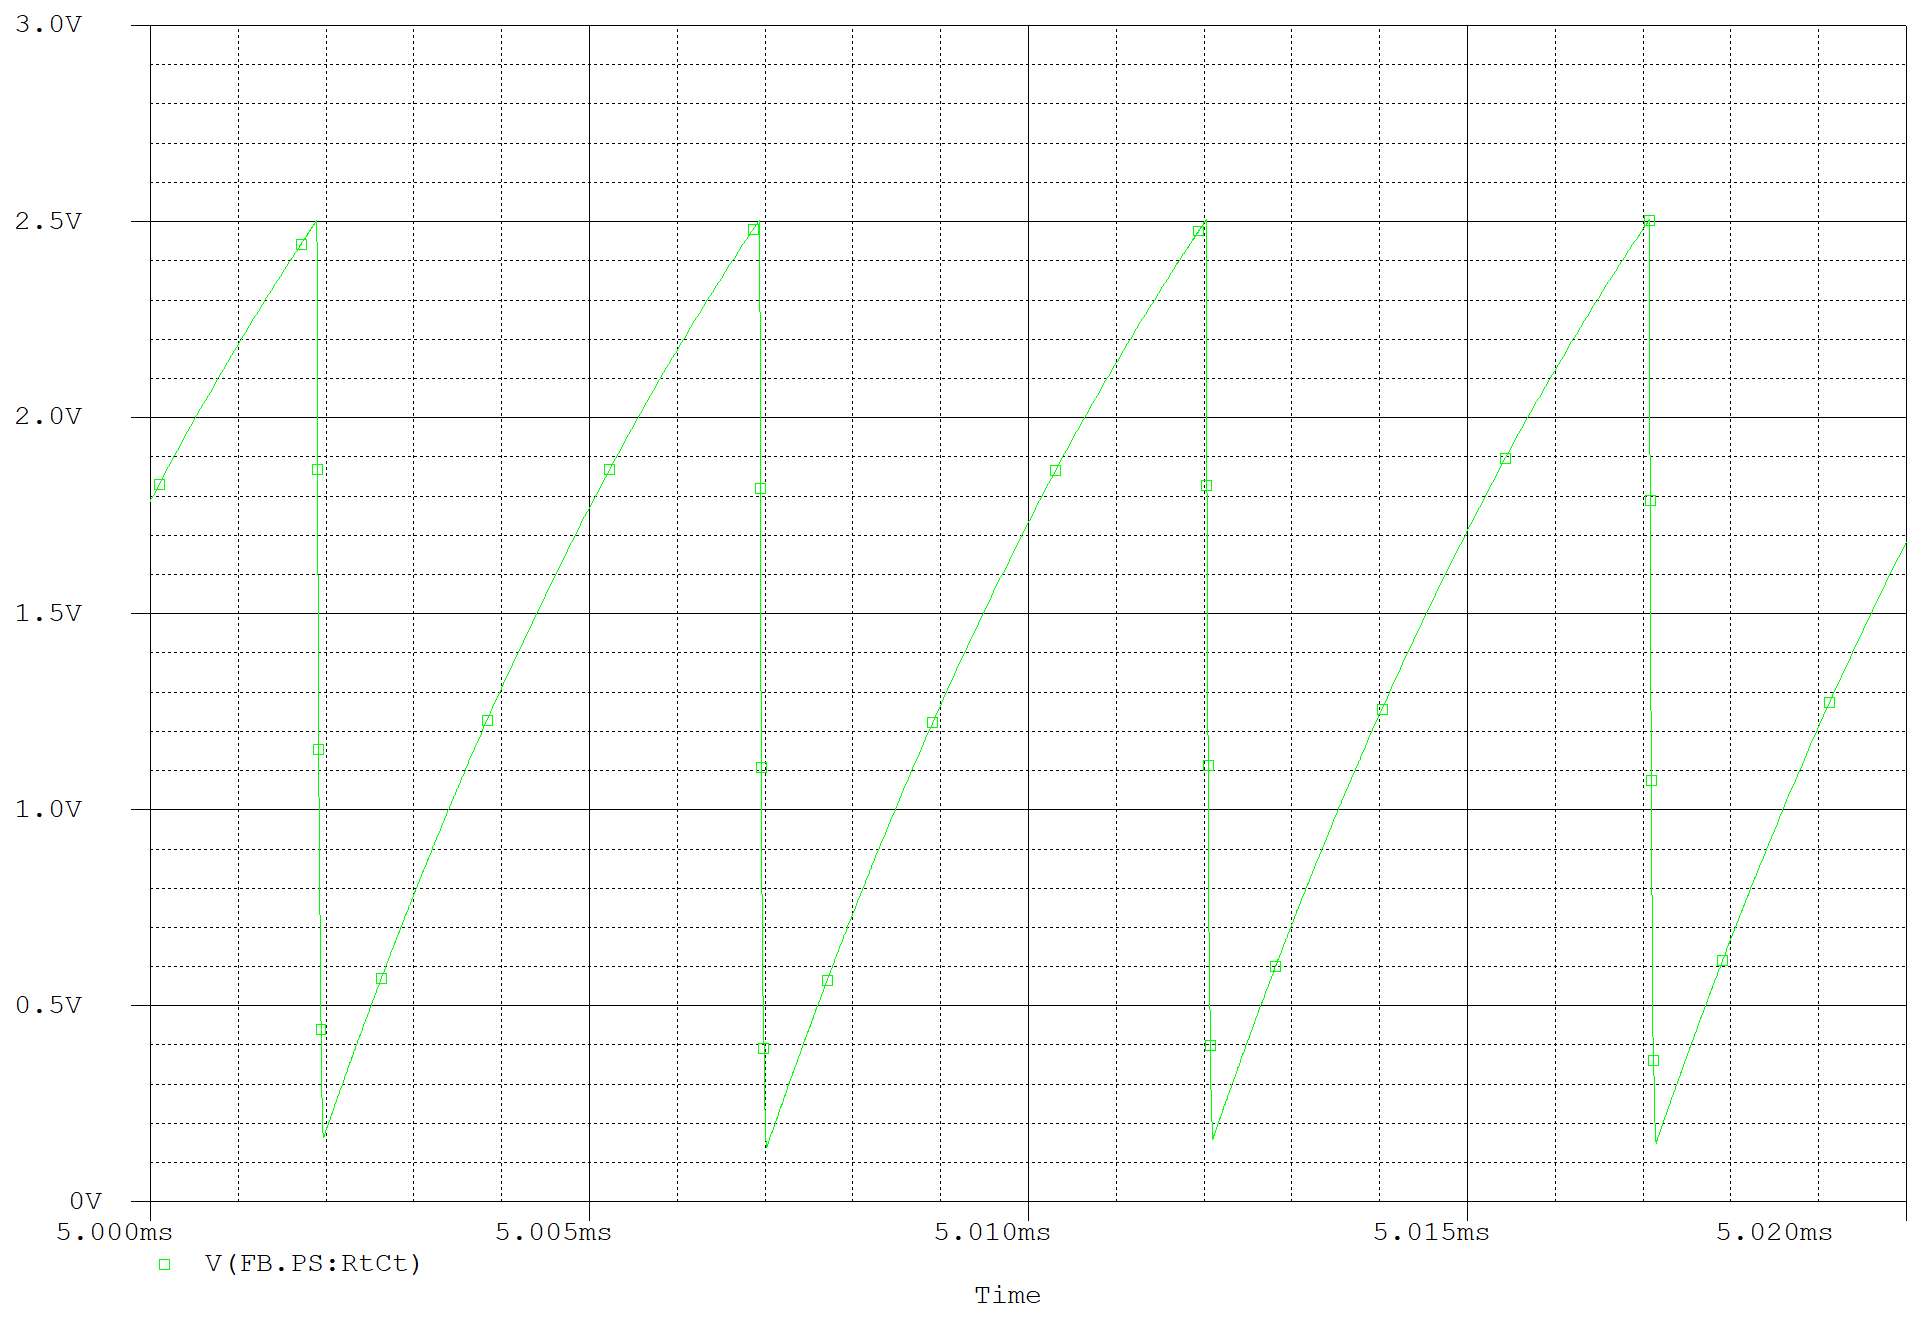
\includegraphics[max width=0.9\linewidth]{/tex/2iteration/billeder/Simulering_PWM_savtand.png}
	\caption{Simulering af savtandspændingen}
	\label{fig:Simulering_PWM_savtand}
\end{figure}

\noindent Nu simuleres selve switch-frekvensen. Dette er gjort på figur~\ref{fig:Simulering_PWM_switch_frekvens}, hvor der måles på udgangen af PWM-controlleren. Her måles periodetiden til $10.1\micro s$, eller en frekvens på $f_s=99.01k\hertz$. 

\begin{figure}[H]
	\center
	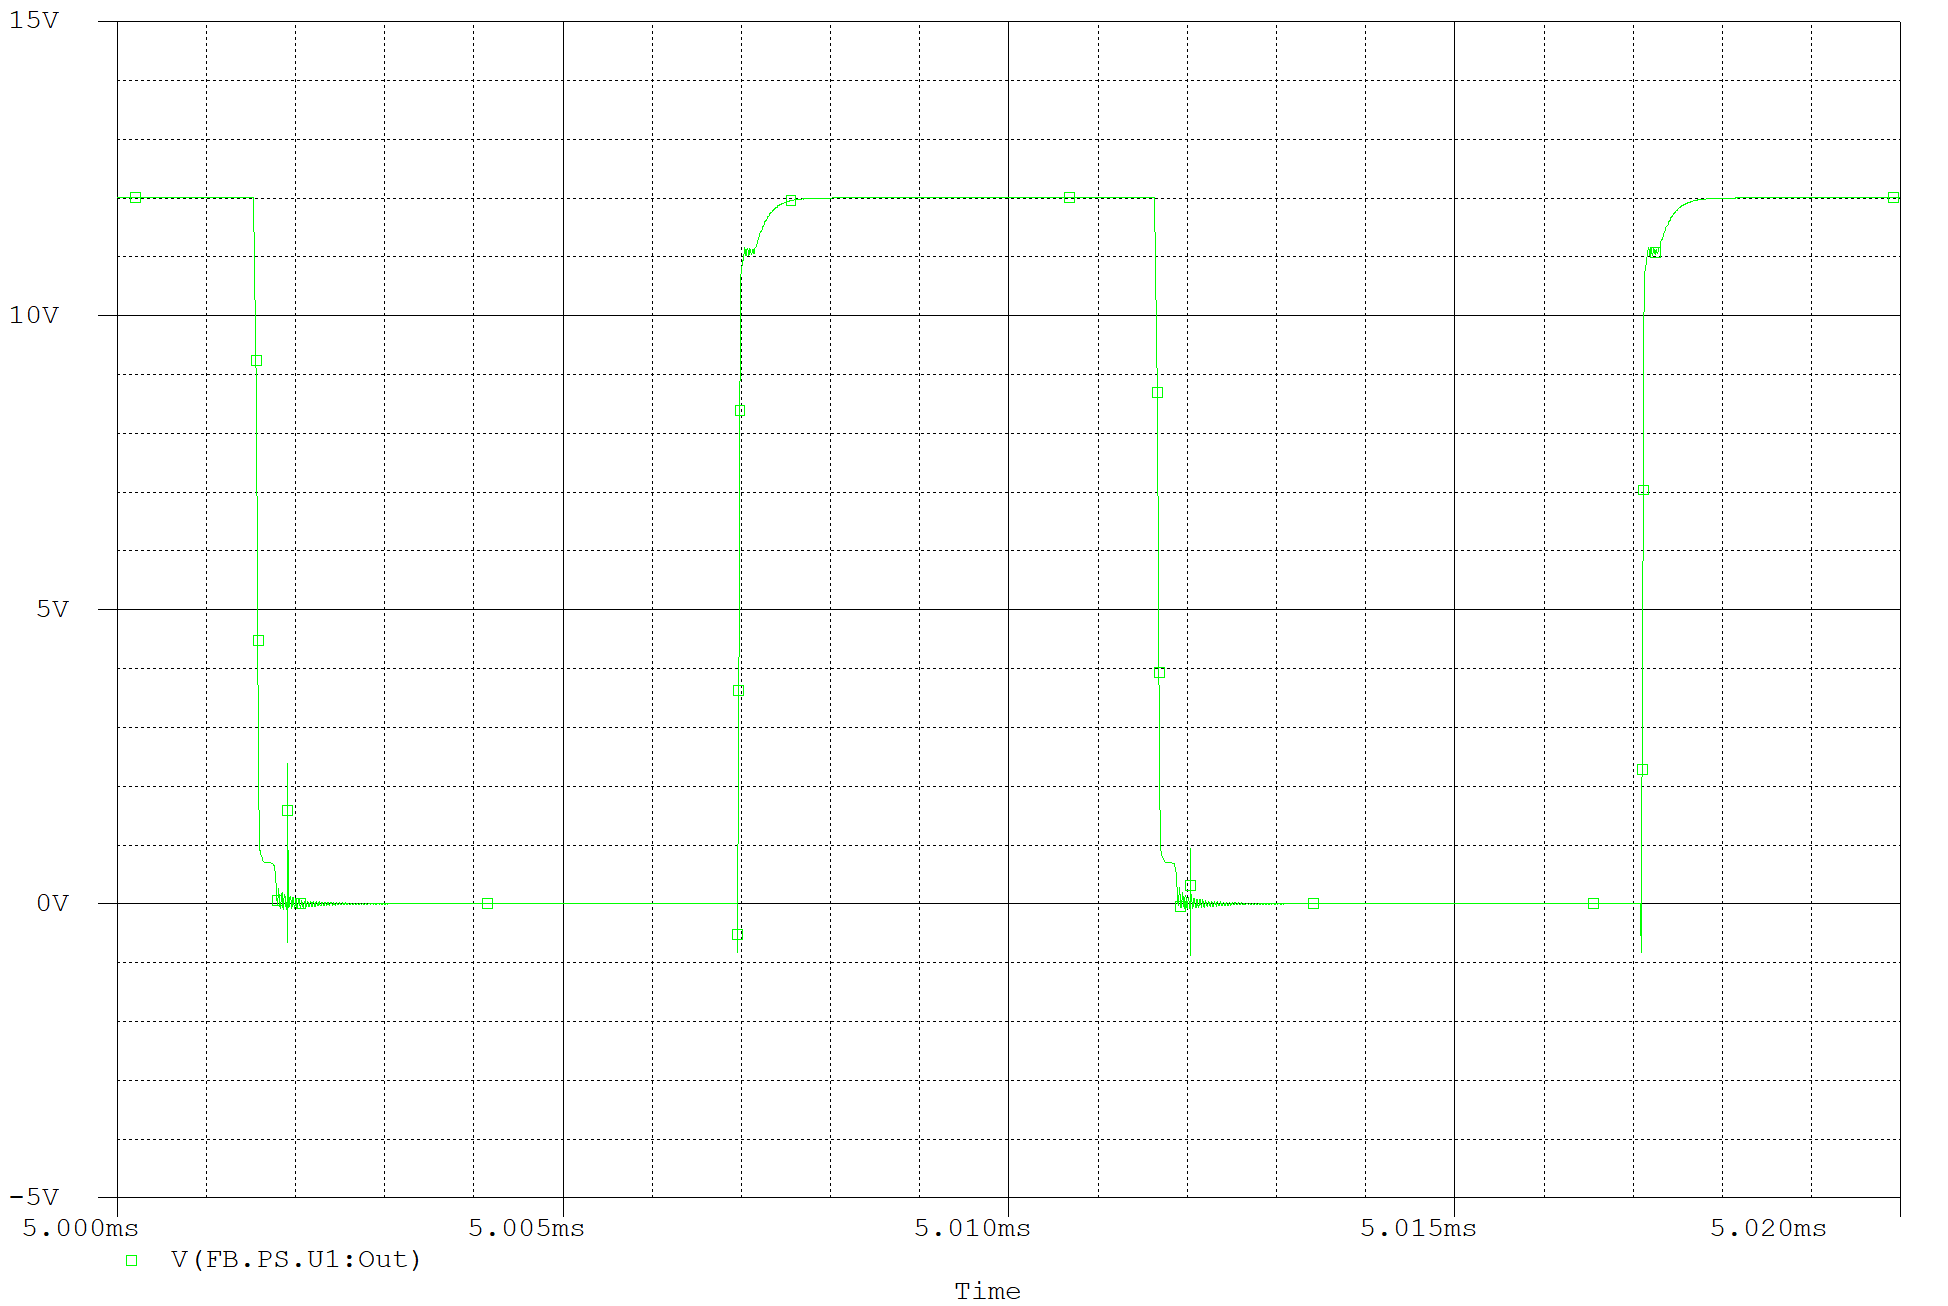
\includegraphics[max width=0.9\linewidth]{/tex/2iteration/billeder/Simulering_PWM_switch_frekvens.png}
	\caption{Simulering af switch-frekvens}
	\label{fig:Simulering_PWM_switch_frekvens}
\end{figure}

\subsubsection{Switch-tid}
\noindent Simuleringen af switch-tiden i MOSFET'en er vist på figur~\ref{fig:Simulering_MOSFET_switch_tid}. Figuren viser et zoom af MOSFET'ens gate signal. Switch-tiden kan aflæses som tiden af signalets plateau. Det aflæses til ca. $103ns$. Grunden til dette afviger meget fra analysen, er modellen for den MOSFET der bruges i simuleringen. Som nævnt bruges en anden MOSFET i simuleringen, end der er regnet med i analysen. En af de specifikationer de afviger mellem de to MOSFETs er \textit{Miller} ladningen, der bruges til at regne switch-tiden. I databladet for IRF630\cite{IRF630}, aflæses den til $15nC$. Regnes switch-tiden ud fra det, fås $107.1ns$, hvilket stemmer med det simulerede. 
\begin{equation} 
T_{ch} = \frac{Q_{gd} \cdot R_{g}}{V_{DD}-V_{gs}} = \frac{15nC \cdot 50\ohm}{12V-5V} = 107.1ns
\end{equation}

\begin{figure}[H]
	\center
	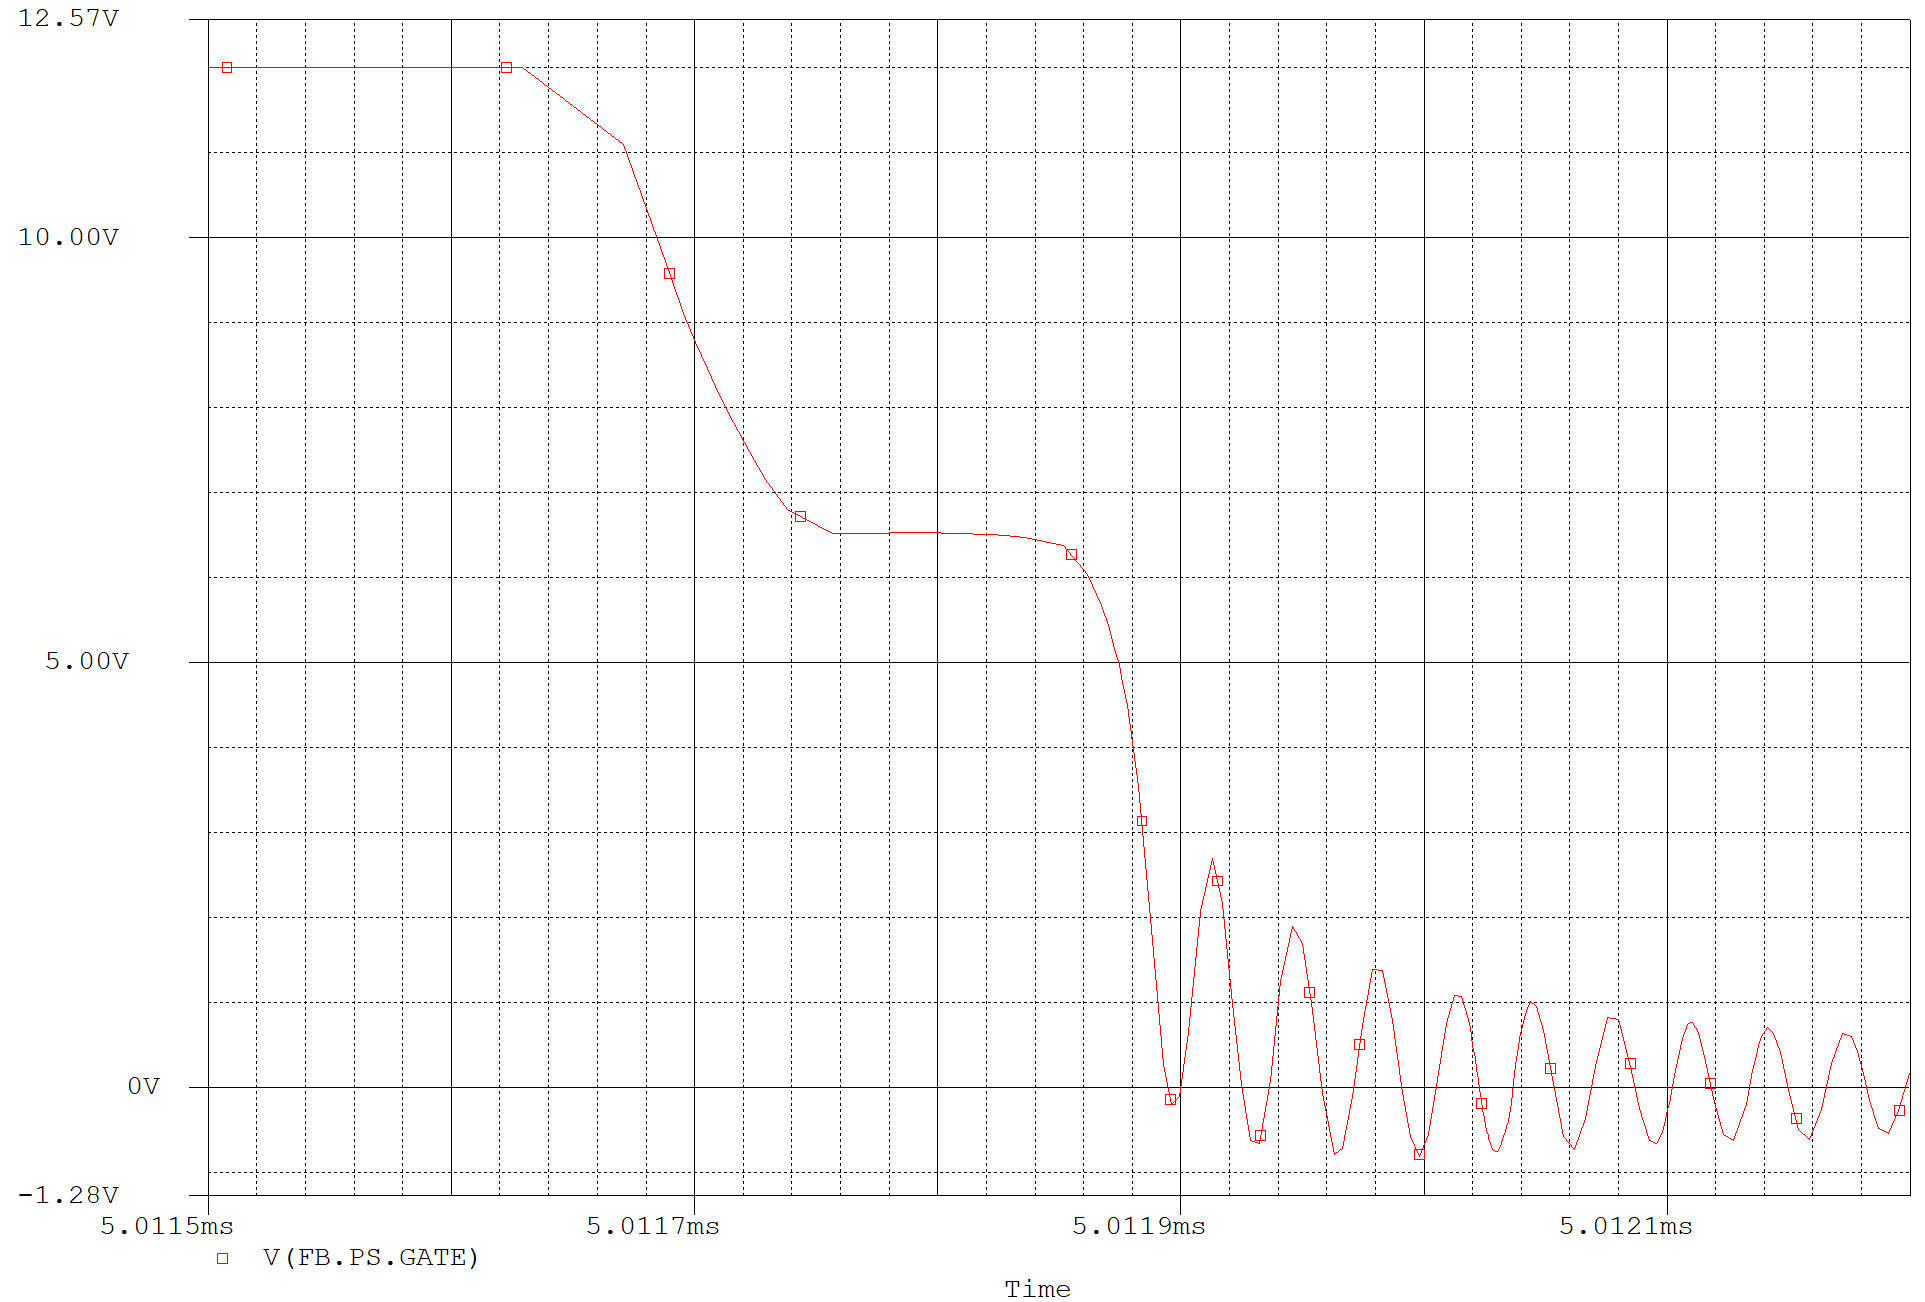
\includegraphics[max width=0.9\linewidth]{/tex/2iteration/billeder/Simulering_MOSFET_switch_tid.png}
	\caption{Simulering af switch-tid i MOSFET}
	\label{fig:Simulering_MOSFET_switch_tid}
\end{figure}


\subsubsection{Current-sense}
\noindent Current-sense signalet måles både før og efter filtreringen. Signalet før filteret ses på figur~\ref{fig:Simulering_PWM_current_sense_U}. Her ses de spikes på signalet, der kan give anledning til en forkert duty-cycle. Figur~\ref{fig:Simulering_PWM_current_sense_M} viser simuleringen for signalet efter filtreringen. Her ses det, at spikesene er blevet filtreret væk, dog med den konsekvens at signalet har fået en langsommere stigetid. Stigetiden aflæses til ca. $280ns$. Ifølge teorien burde PWM-controllerens udgangssignal skifte, når current-sense signalet er lig $1V$. På figur~\ref{fig:Simulering_PWM_current_sense_M}, ses det, at dette også er tilfældet for p-spice modellen for UCC1801. 


\begin{figure}[H]
	\center
	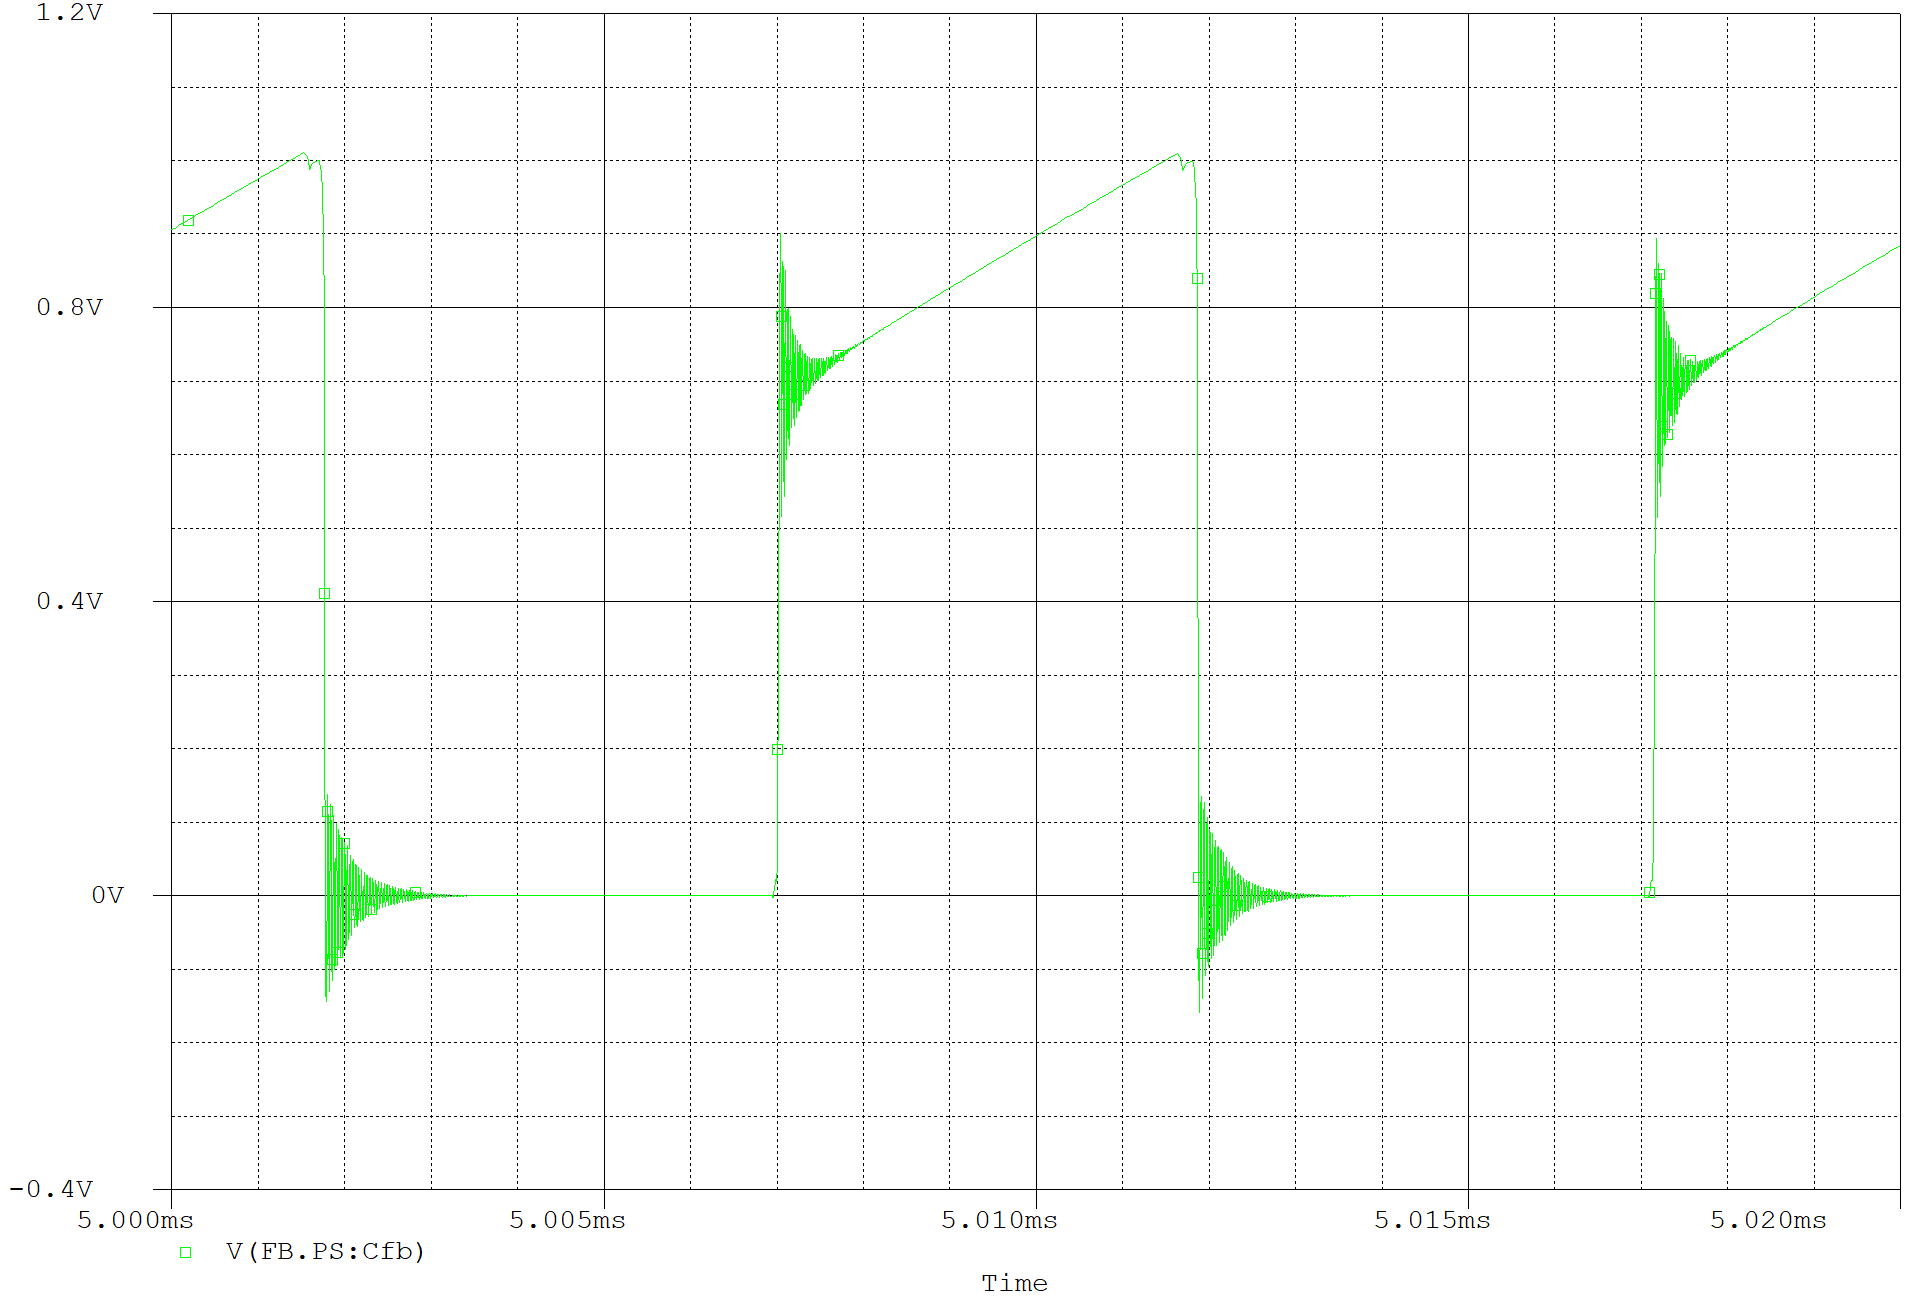
\includegraphics[max width=0.9\linewidth]{/tex/2iteration/billeder/Simulering_PWM_current_sense_U.png}
	\caption{Simulering af current-sense signal før filtrering}
	\label{fig:Simulering_PWM_current_sense_U}
\end{figure}

\begin{figure}[H]
	\center
	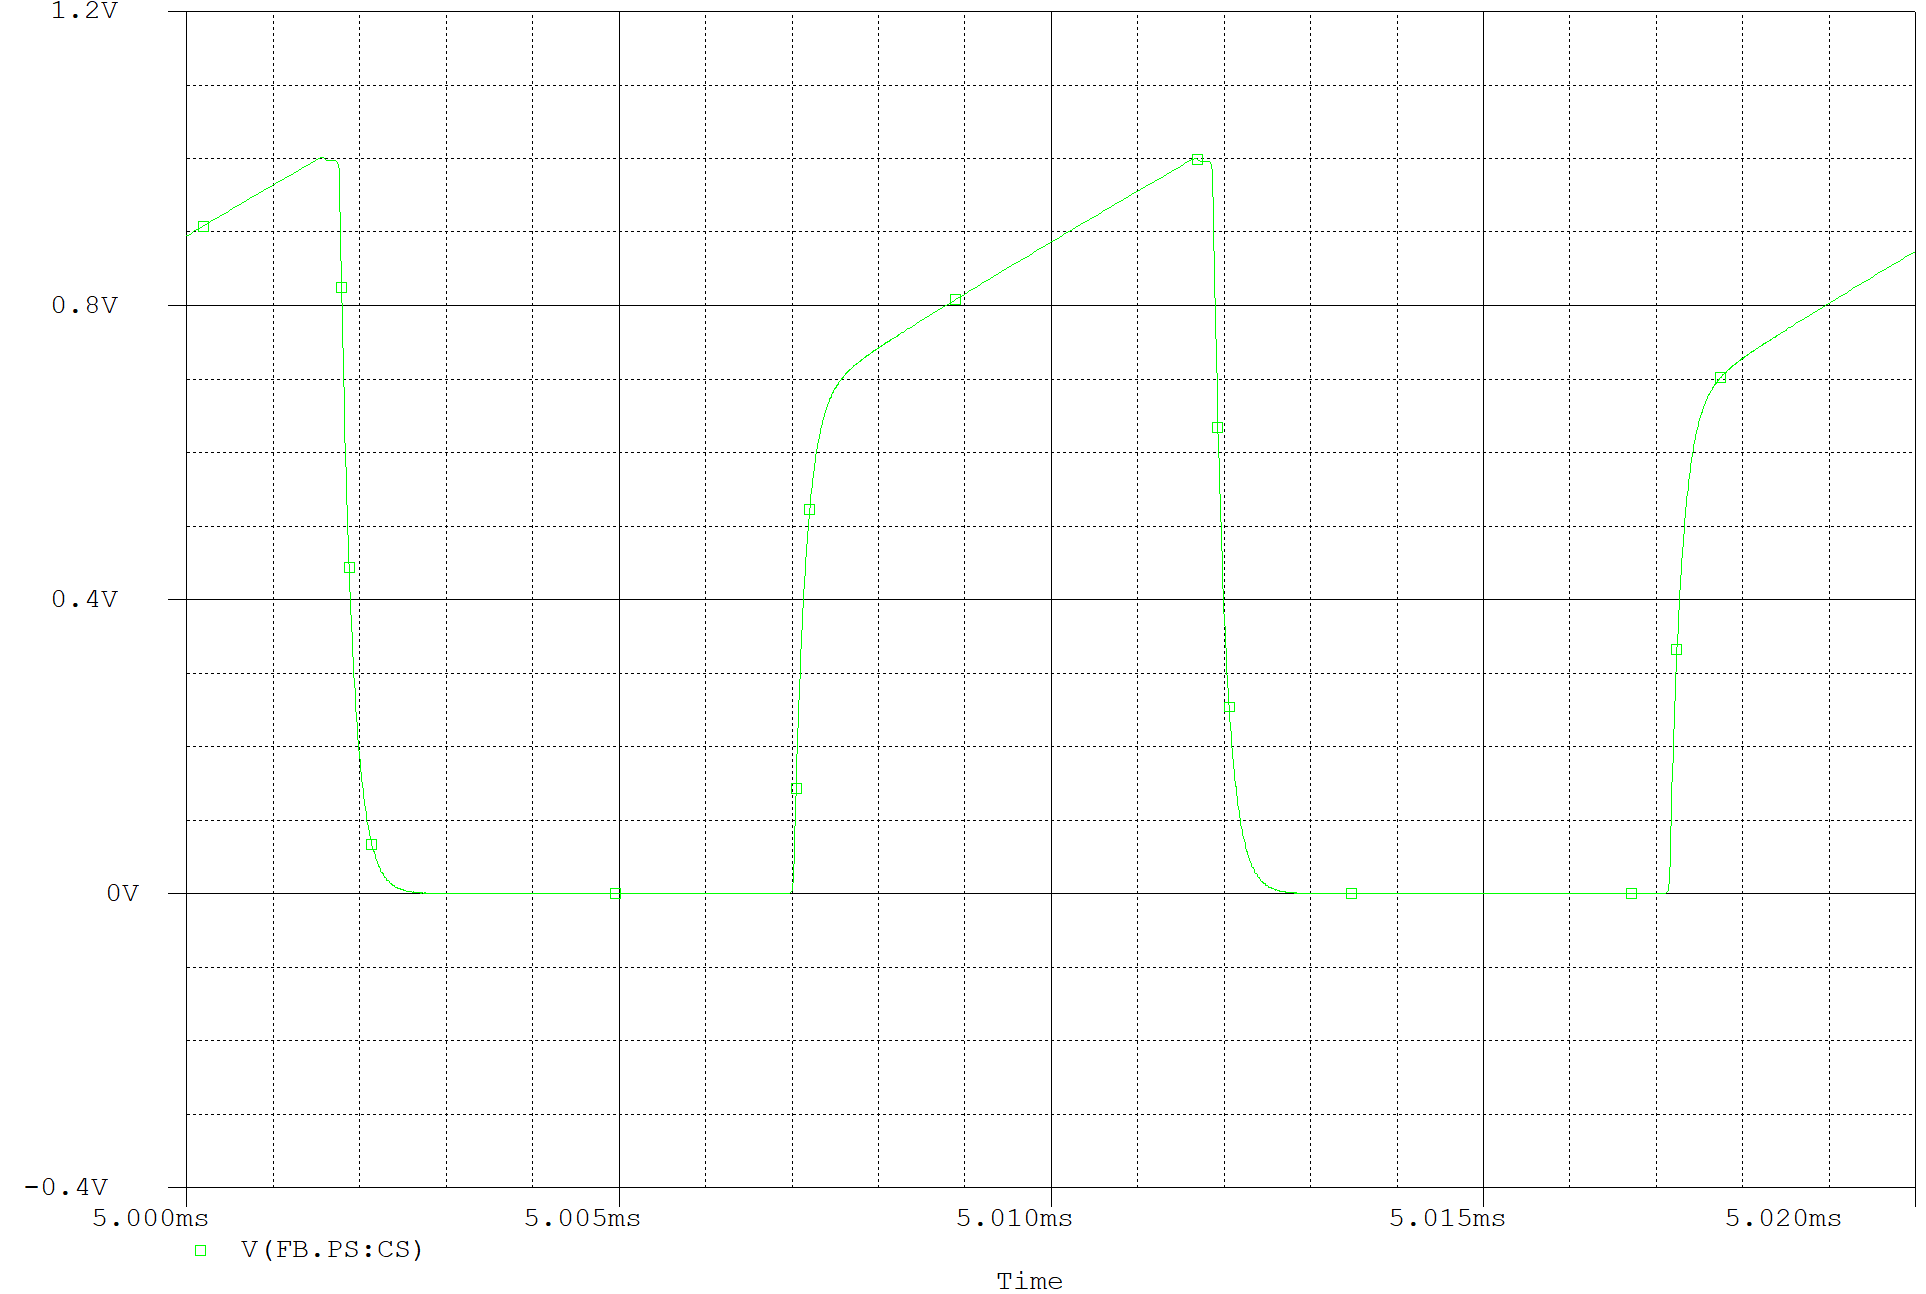
\includegraphics[max width=0.9\linewidth]{/tex/2iteration/billeder/Simulering_PWM_current_sense_M.png}
	\caption{Simulering af current-sense signal efter filtrering}
	\label{fig:Simulering_PWM_current_sense_M}
\end{figure}




\subsection{Constant load} \label{constant}
Ved constant load simuleringen simuleres ved en load på $8.4\ohm$, efter $20ms$ så det sikres, at der ses på den stationære udgang. Indgangsspændingen er sat til 26V.
Første plot af denne simulering ses på figur~\ref{fig: simflycon}. Her ses både strøm og spænding på udgangen.
\begin{figure}[H]
	\center
	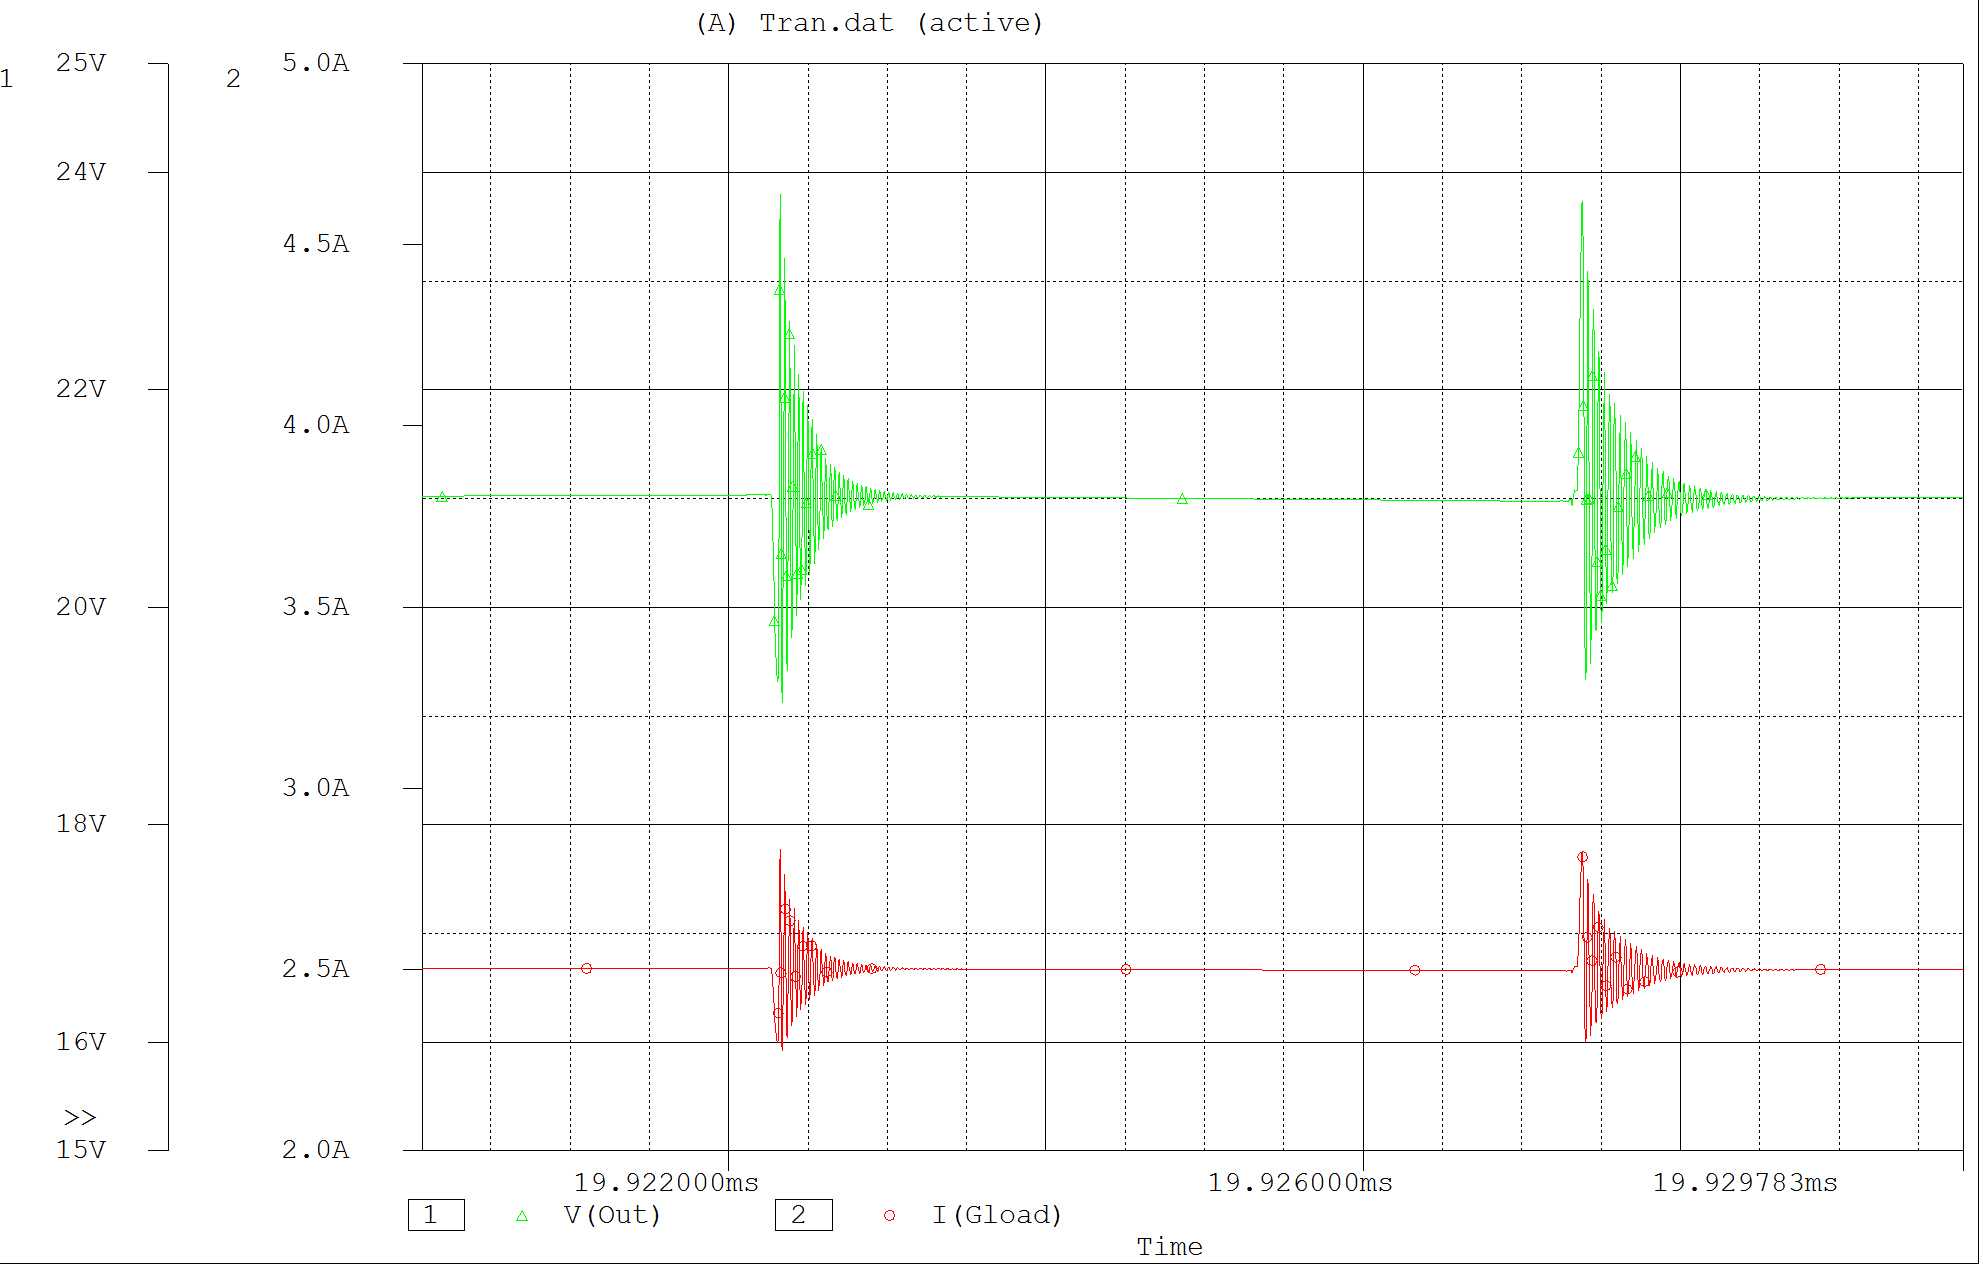
\includegraphics[max width=0.7\linewidth]{/tex/2iteration/billeder/Simudgang.png}
	\caption{Simulering af udgang}
	\label{fig: simudgang}
\end{figure}
Her ses det at spændingen V(out) ligger på 21V, dog med svingninger hver gang der switches. Det ser altså ud til at switching transienter fra MOSFET og diode kommer til syne på udgangen. Det er samme billede for strømmen I(Gload), der ellers ligger på de forventede 2.5A.

På figur~\ref{fig: simMOSdio} ses en spændingsperiode for drain benet på MOSFET'en samt dioden. 
\begin{figure}[H]
	\center
	\includegraphics[max width=0.7\linewidth]{/tex/2iteration/billeder/SIMMOSFETdiode.png}
	\caption{Simulering af spænding over diode og drain ben på MOSFET}
	\label{fig: simMOSdio}
\end{figure}
Det ses, at når transistoren (rød kurve) går off så kommer den tidligere omtalte peakspænding samt den svinger, inden den går til en stationær værdi på ca. 48V, inden MOSFET'en switches on igen. Dette stemmer fint overens med analysen hvor den stationær værdi bør ligge på 21V+26V=47V.
Peak'en er ca. 93V.
Det samme ses for dioden (grøn kurve) at når transistoren er on, vil dioden ikke være i lederetningen, og skal derfor kunne holde til den peak på ca. 80V der ses på grafen. Derudover lægger den sig på en stationær værdi på ca. 46V, hvilket igen stemmer pænt overens med de 47V. 

På figur~\ref{fig: simMOSzoom} zoomes der ind på svingningerne på MOSFET'ens drain.
\begin{figure}[H]
	\center
	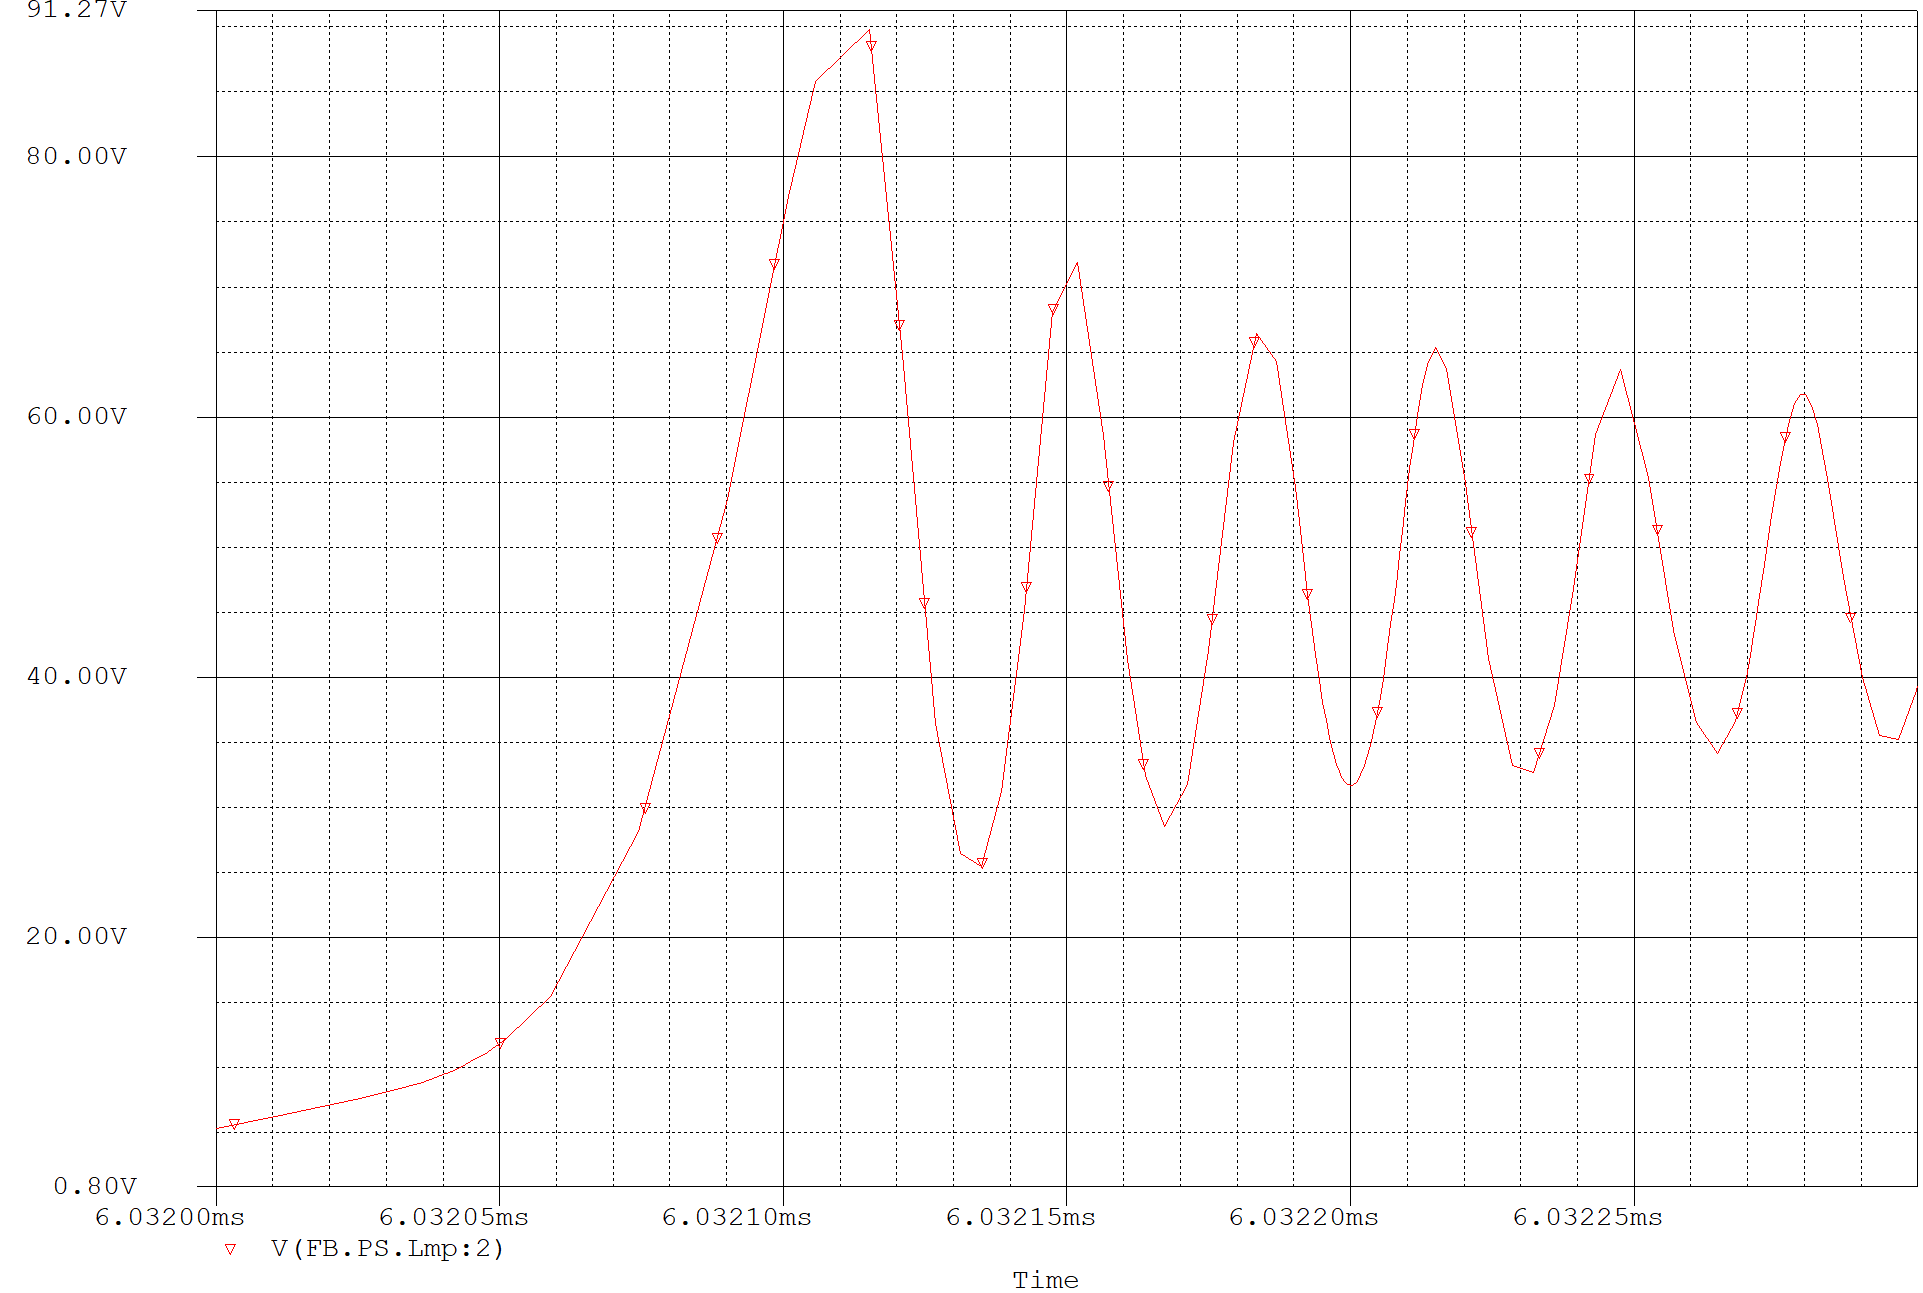
\includegraphics[max width=0.7\linewidth]{/tex/2iteration/billeder/Simulering_MOSFET_drain_zoom.png}
	\caption{Zoomet simulering af svingninger fra MOSFET}
	\label{fig: simMOSzoom}
\end{figure}
Her kan svingningernes frekvens aflæses. Det gøres ved, at aflæse længden på en svingning. Her er anden svingning aflæst til 34ns. Det giver en frekvens på 29.41MHz.

Det samme gøres for det zoomede billede af svingningerne i dioden som ses på figur~\ref{fig: simdiodezoom} 
\begin{figure}[H]
	\center
	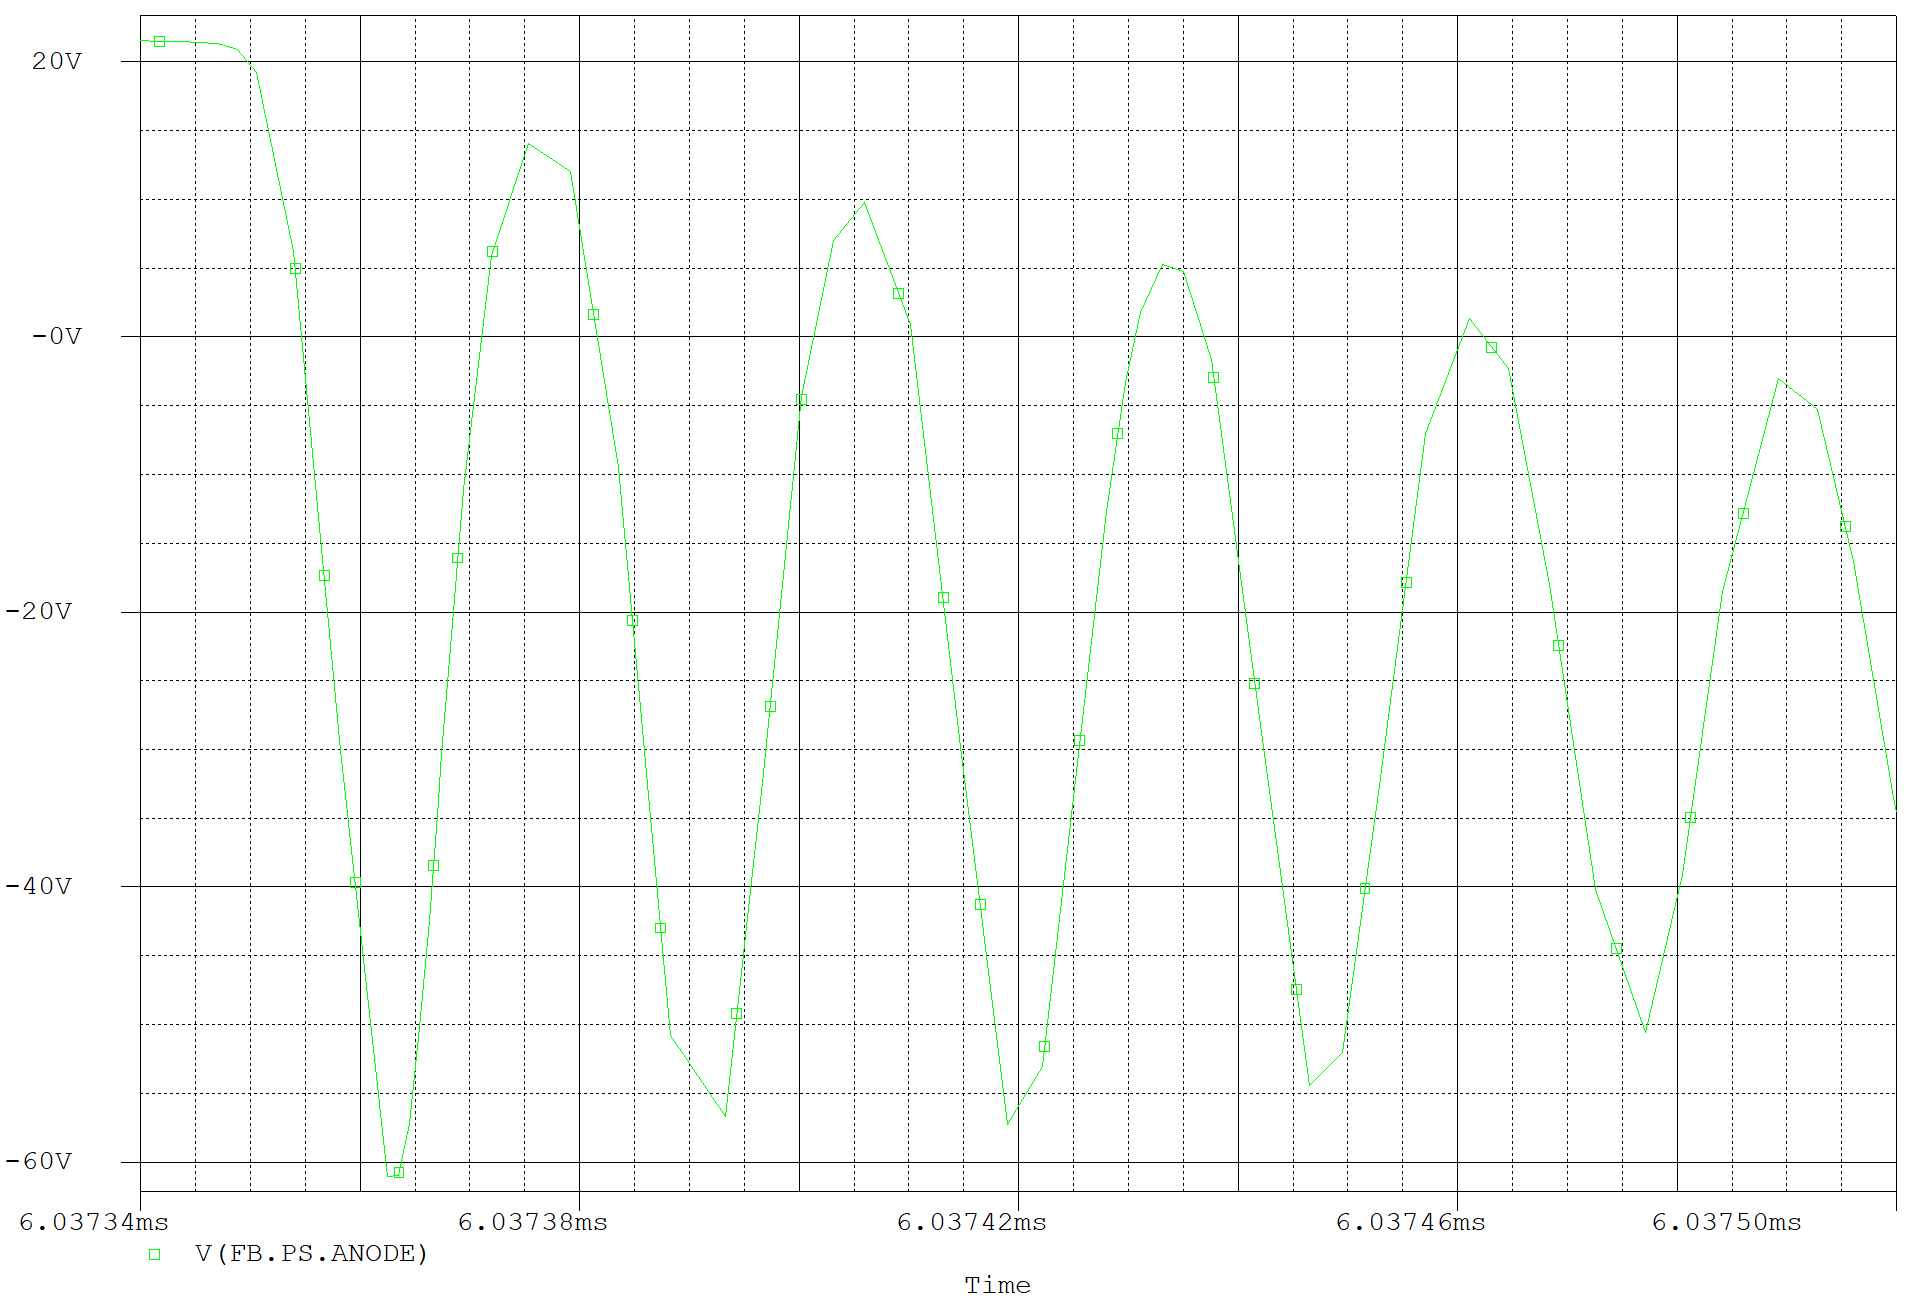
\includegraphics[max width=0.7\linewidth]{/tex/2iteration/billeder/Simulering_diode_anode_zoom.png}
	\caption{Zoomet simulering af svingninger fra diode}
	\label{fig: simdiodezoom}
\end{figure}
Anden svingning er her aflæst til 30ns. Det giver en frekvens på $33.33M\hertz$

\subsection{Load step}
Ved load steppet kontrolleres det, hvor hurtigt systemet får reguleret ind efter en ny load. I forhold til før, er der sket en ændring i toplaget i schematic, som ses på figur~\ref{fig: simloadtop}  
\begin{figure}[H]
	\center
	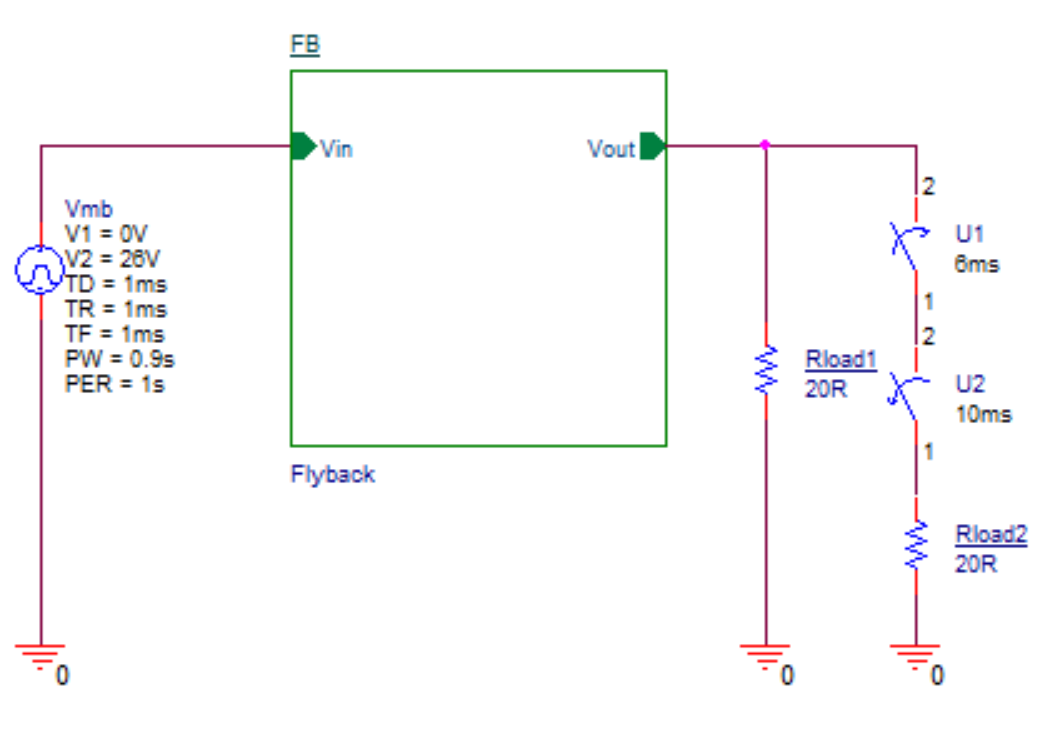
\includegraphics[max width=0.7\linewidth]{/tex/2iteration/billeder/Simloadtop.png}
	\caption{Toplaget for simulering af load step}
	\label{fig: simloadtop}
\end{figure}
Den eneste forskel er i udgangsloaden. Som her består af 2 $20\ohm$ modstande i parallel, hvor den ene sidder for enden af 2 switches. Switchen U1 åbner efter 21ms hvor begge switches vil være on. Her er loaden parallelmodstanden af Rload1 og Rload2 og dermed $10\ohm$. Dette sker i 4ms, indtil switch U2 lukker og loaden igen består af de $20\ohm$ fra Rload1.

\noindent Udover dette er der en yderligere ændring. Ved denne simulering er parasit spolen fjernet fra udgangskondensatoren. Dette er gjort, da spolen som før set, giver anledning til en del svingninger. Det er ikke den del, der her i load steppet er interessant, og derfor ses der bort fra den. Det vigtige er istedet hvor hurtigt der bliver reguleret og hvor stort et overshoot der fås. Simuleringsresultatet ses på figur~\ref{fig: simloadstep} 

\begin{figure}[H]
	\center
	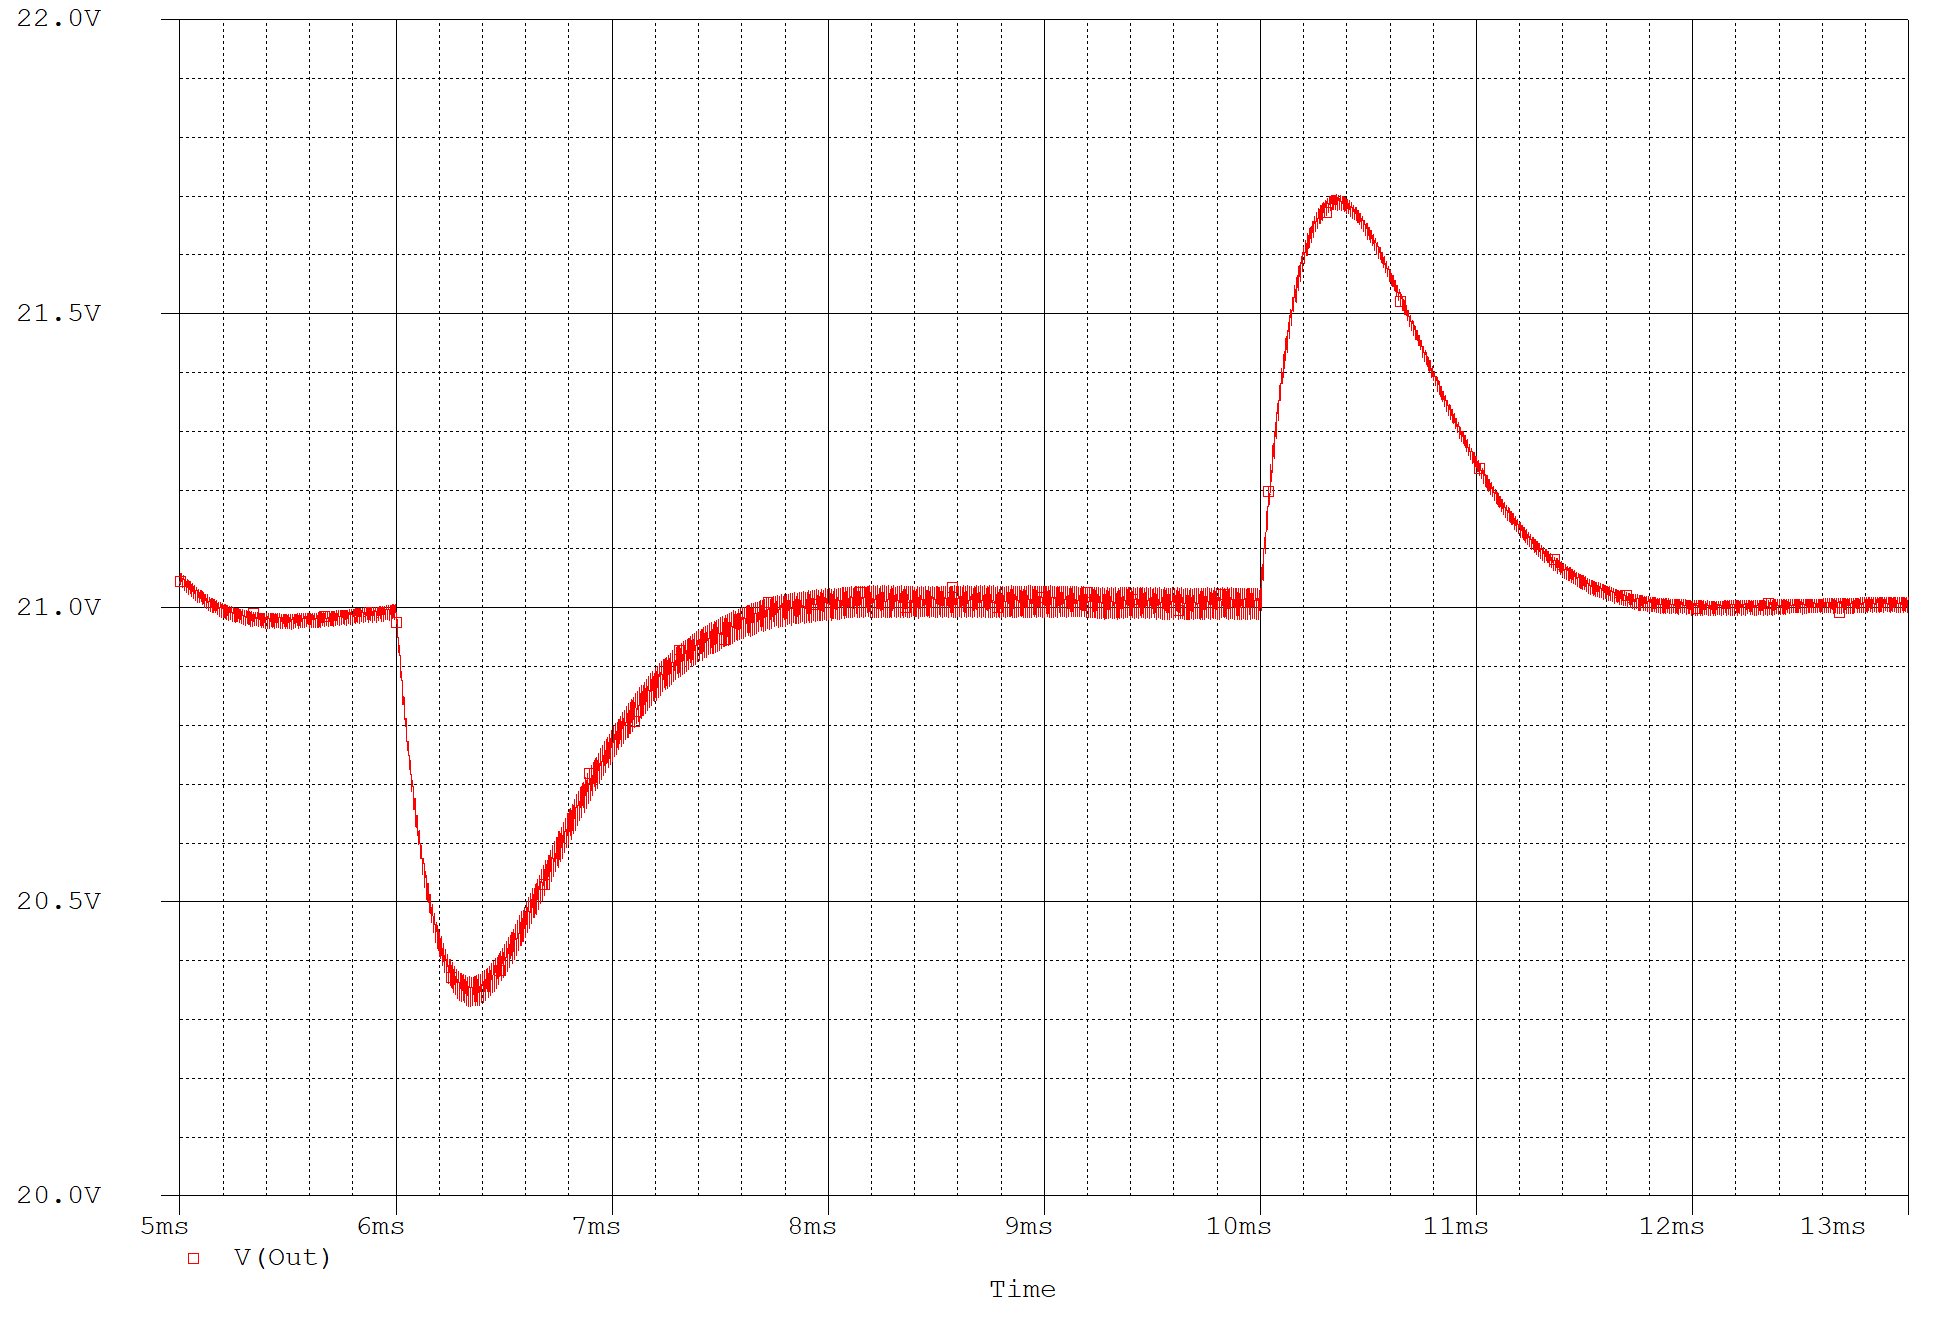
\includegraphics[max width=0.7\linewidth]{/tex/2iteration/billeder/Load_step_simulering.png}
	\caption{Simulering af load step}
	\label{fig: simloadstep}
\end{figure}

Det ses, at så snart switch U1 går on falder spændingen fra $21V$ til ca. $20.35V$ og det tager systemet ca. 1.6ms at regulere tilbage igen. Da U2 går off stiger spændingen fra 21V til 21.7V og bruger igen 1.6ms, på at regulere spændingen tilbage til de 21V. 

\subsection{Startup}
Ved startup er schematic sat op på præcis samme måde som ved Constant load. Forskellen er her, at der ved simuleringen ses fra 0ms til 20ms. På den måde ses det hvordan systemet starter op, og hvor hurtigt der reguleres ind på de 21V. Da der er koblet en direkte spændingskilde på 12V ind på VCC for PWM controlleren, får man ikke det endelige billede af, hvordan det færdige vil se ud. Det bruges istedet for til at se, hvor hurtigt der reguleres ind, og om der sker nogle uforudsete ting under simuleringsstarten.
 Simuleringsresultatet ses på figur~\ref{fig: simloadstep} 

%%% Simulering for optimering af reguleringsloop %%%

\subsection{Gain-fase}
Simuleringen af systemets gain-fase karakteristik, udføres på samme måde som ved 2. iteration. Bode plot for fejlforstærkeren er vist på figur~\ref{fig:Simulering_error_op_amp_3}. Da knækfrekvensen for fejlforstærkeren ligger ved $132\hertz$, og der ikke kan simuleres med frekvenser lavere end $100\hertz$, er det svært at aflæse bode plottet. Det kan dog aflæses, at forstærkningen over $132^\circ$ ligger sig på ca. $8.6\decibel$. Derudover ses det at fasen stiger til $180^\circ$, derfor antages det, at fejlforstærkeren vil bidrage med det forventede faseløft på $90^\circ$. 

\begin{figure}[H]
	\center
	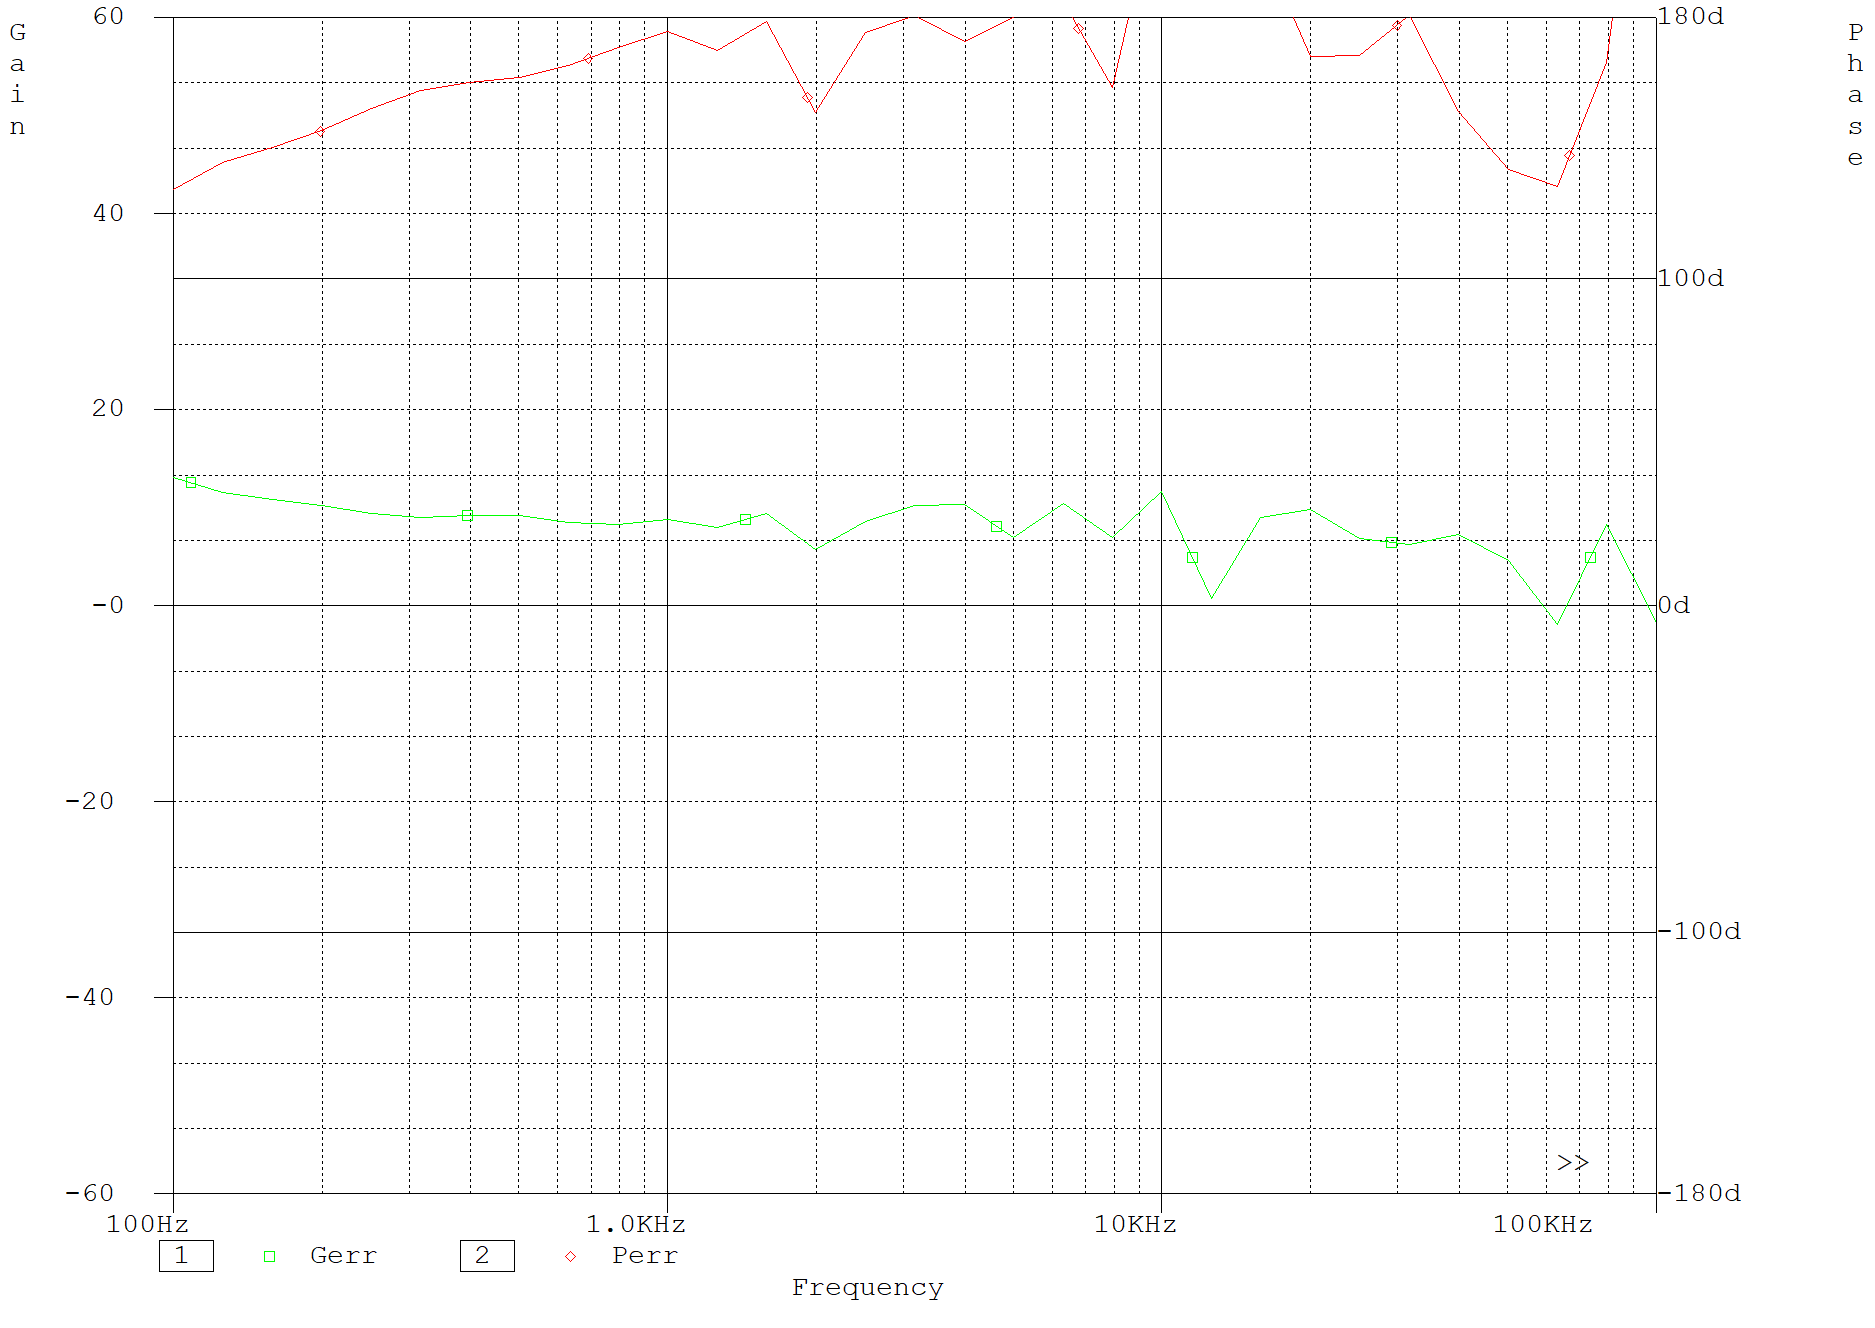
\includegraphics[max width=0.9\linewidth]{/tex/3iteration/billeder/Simulering/Simulering_error_op_amp.PNG}
	\caption{Simulering af fejlforstærkeren}
	\label{fig:Simulering_error_op_amp_3}
\end{figure}

\noindent Bode plottet for det samlede system er vist på figur~\ref{fig:Simulering_total_3}. Selvom simuleringen bliver usikker ved høje frekvenser, sker det så langt oppe i frekvens, at de relevante værdier akkurat kan aflæses. Gain-margin aflæses til ca. $10.2\decibel$, fase-margin aflæses til ca. $73.2^\circ$, og båndbredden aflæses til ca. $3.5k\hertz$. Ift. analysen passer både gain- og fasemargin, mens båndbredden ca. $400\hertz$ lavere end det forventede. 

\begin{figure}[H]
	\center
	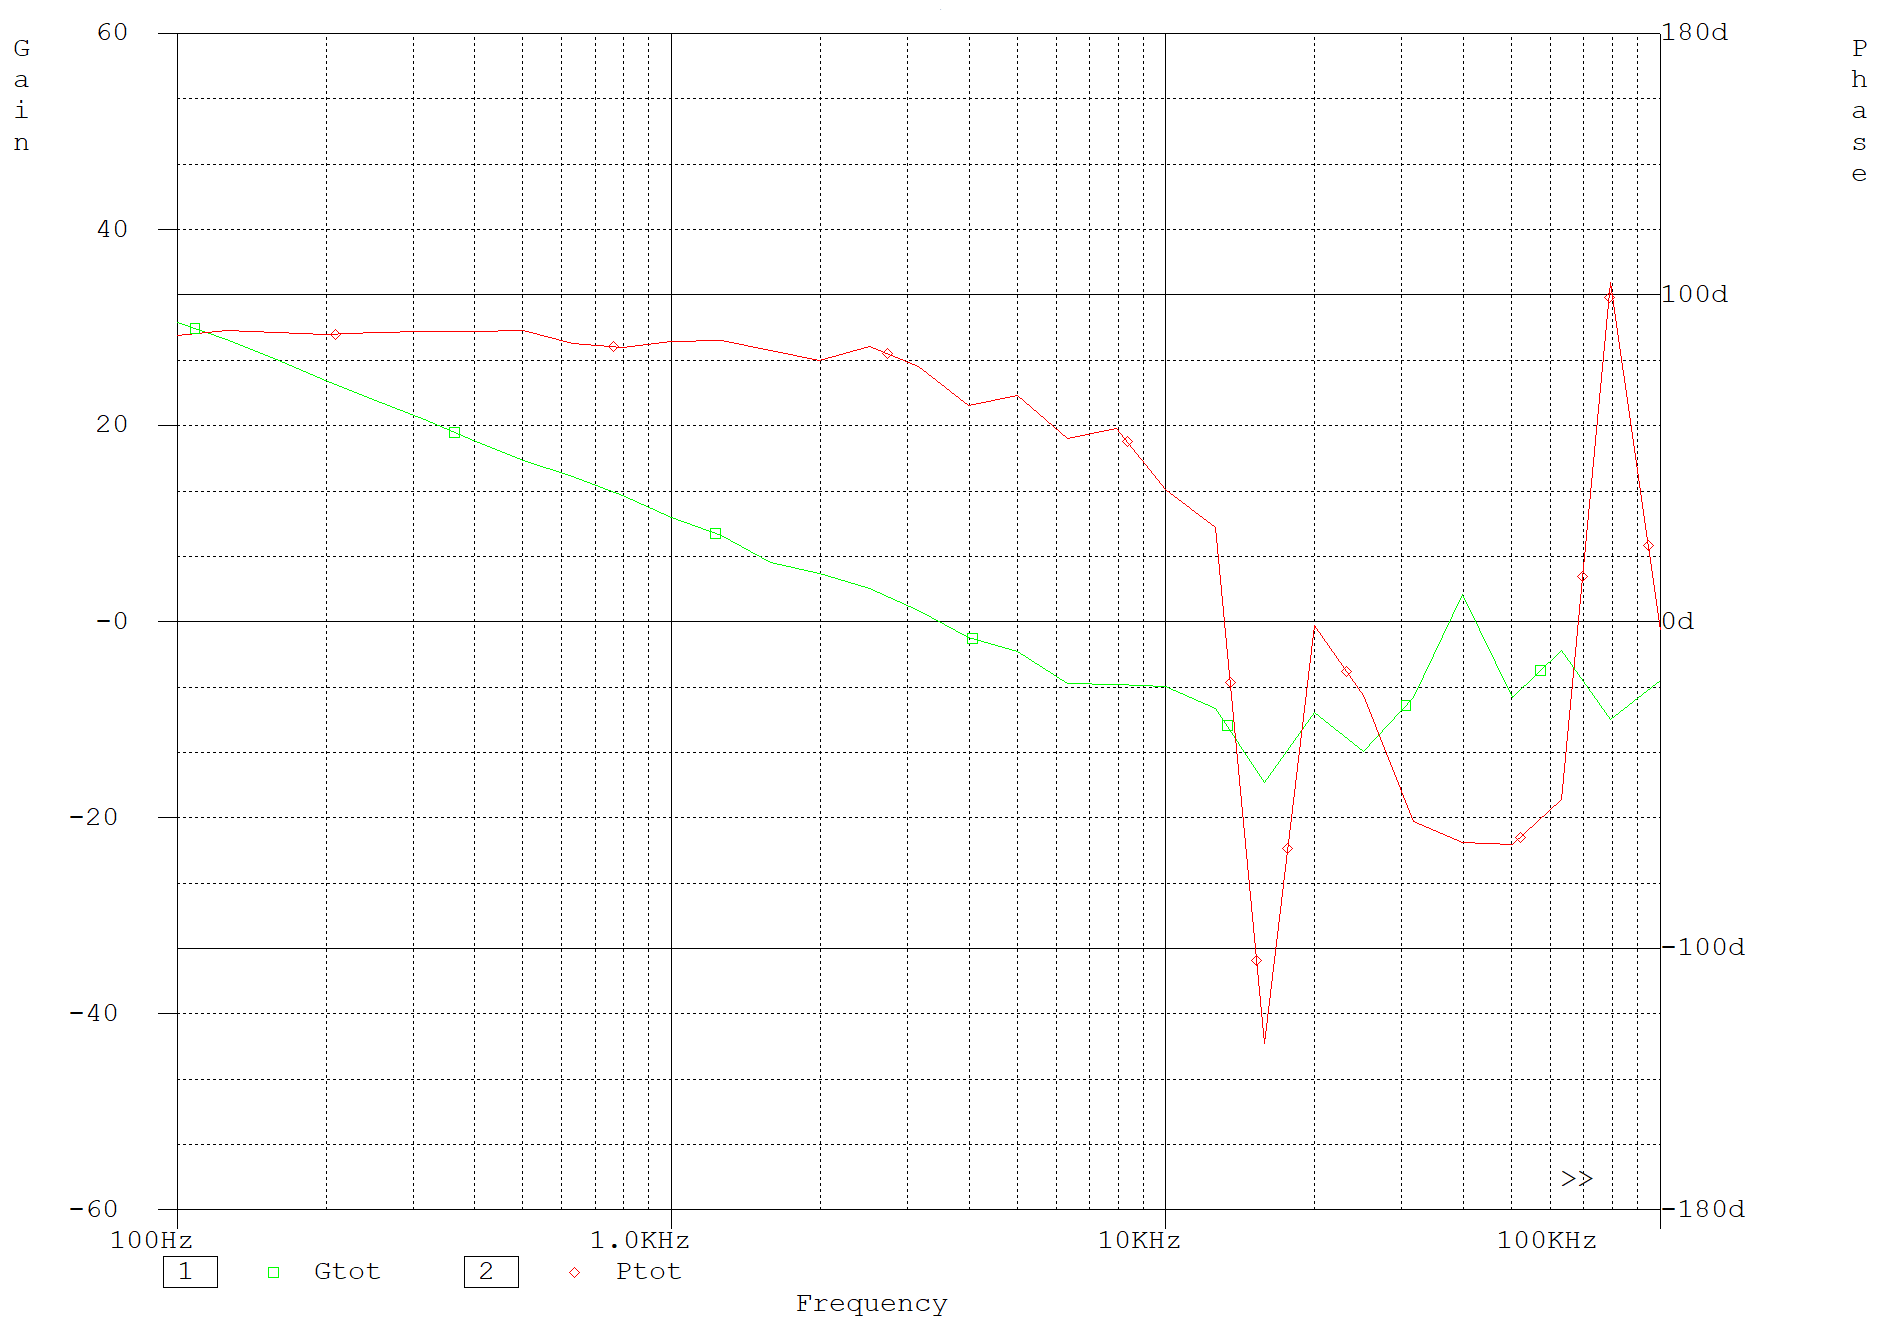
\includegraphics[max width=0.9\linewidth]{/tex/3iteration/billeder/Simulering/Simulering_total.PNG}
	\caption{Simulering af det samlede system}
	\label{fig:Simulering_total_3}
\end{figure}  

\subsection{Tab}
Her er tabene for de forskellige komponenter simuleret, ligesom de blev analyseret tidligere.

\subsubsection{Transformator}
Kernetabet i transformatoren er simuleret tidligere ~\ref{Simkernetab} til $311m\watt$. Der er indsat modstande på $53.33\ohm$ på både primær- og sekundærsiden af transformatoren for at simulere det analyserede kobbertab. På figur~\ref{fig: simloadstep} ses det simulerede kobbertab. Her er der lavet en average på de 2 kobbermodstande lagt sammen. 
Dt ekstra tab der er simuleret i forhold til analysen kommer af at spredningsselvinduktionen er indsat i simuleringsprofilen. Det får RMS strømmen på primær og sekundær til at stige, og ligger dermed på et højere niveau end den analyserede værdi????
\subsubsection{MOSFET}
Conduction og switchtab er her simuleret. figur~\ref{fig: simloadstep} ses tabet for hver periode. Det ses at der kommer de førnævnte effekttrekanter når der switches. Det er det simulerede switchtab. Offsettet imellem disse effekttrekanter er conduction tabet.
På figur~\ref{fig: simloadstep} er der lavet en average af simuleringen. Det giver det samlede tab for både conduction og switchtab. Det aflæses til at ligge på. Tabet her ligger lidt under det analyserede. Det skyldes at modellen der er brugt i simuleringen, ikke er den samme som bruges i analyse og realisering. Samtidig er analysen et estimat af tabet, hvor der foreksempel regnes med at effekttrekanterne er lige store. Begge dele kan være fejlkilder der gør, at de to tab ikke stemmer helt overens.  

\subsubsection{Diode}
Diodens tab er simuleret på figur~\ref{fig: simloadstep}. Tabet aflæses til .. Grunden til det ikke stemmer så godt overens med det analyserede skyldes at modellen regner med et spændingsfald på $0.6V$, hvor der i analysen er brugt $0.45V$. Dette kommer af at simuleringsmodellen ikke tager højde for at spændingsfaldet ændrer sig med strømmen og temperaturen. 

\subsubsection{Samlet tab}
\begin{table}[H] 			
	\centering
	\begin{tabularx}{\textwidth}{|X|l|l|}
		\hline
		\textbf{\large Komponent} & \multicolumn{2}{|X|}{\textbf{\large Tab}} \\ \hline
		& A & S	\\ \hline
		\textbf{Transformator samlet} & $2.04\watt$ & \\ \hline 
		Kernetab & $366m\watt$ & $311m\watt$ \\ \hline
		Kobbertab & $1.09\watt$ & \\ \hline
		& &	\\ \hline
		\textbf{MOSFET samlet} & $5.55\watt$ & \\ \hline
		Conductiontab & $1.06\watt$ & \\ \hline
		Switchtab & $4.49\watt$ & \\ \hline
		& &	\\ \hline
		\textbf{Diode} & $1.13\watt$ & \\ \hline
		& &	\\ \hline
		\textbf{Total tab} & $8.72\watt$ & \\ \hline
	\end{tabularx}
	\caption{Oversigt over analyseret og simuleret tab}
	\label{tab:anasim}
\end{table}